\pdfminorversion=7
\documentclass[aspectratio=169,11pt]{beamer}

\IfFileExists{beamerthemeCCM.sty}{%
  \usetheme{CCM}
}{%
  \usetheme{default}
  \definecolor{CCMorange}{HTML}{F6862D}
  \definecolor{SFdark}{HTML}{1D2954}
  \definecolor{mygray}{HTML}{8F8F8F}
  \setbeamertemplate{navigation symbols}{}
  \setbeamertemplate{footline}[frame number]
  \setbeamersize{text margin left=0.25in,text margin right=0.25in}
  \setbeamercolor{title}{fg=CCMorange}
  \setbeamercolor{frametitle}{fg=CCMorange,bg=white}
  \setbeamercolor{item}{fg=CCMorange}
  \setbeamercolor{block title}{fg=black,bg=CCMorange!30}
  \setbeamercolor{block body}{fg=black,bg=black!3}
}

\usepackage{amsmath,amssymb,mathtools}
\usepackage{bm}
\usepackage{booktabs}
\usepackage{graphicx}
\usepackage{times}
\usepackage{tikz}
\usepackage{url}
\usetikzlibrary{arrows.meta,calc,positioning,decorations.pathreplacing}

% Colors used in the source-derived Estrin pipeline animation.
\definecolor{estrinXtwo}{RGB}{25,25,25}
\definecolor{estrinXfour}{RGB}{31,120,180}
\definecolor{estrinU}{RGB}{51,160,44}
\definecolor{estrinV}{RGB}{251,154,153}
\definecolor{estrinW}{RGB}{227,26,28}
\definecolor{estrinP}{RGB}{253,191,111}
\definecolor{estrinQ}{RGB}{255,127,0}
\definecolor{estrinR}{RGB}{106,61,154}
\definecolor{estrinFinal}{RGB}{177,89,40}

\graphicspath{{day1_morning_figures/}}

\newcommand{\R}{\mathbb{R}}
\newcommand{\C}{\mathbb{C}}
\newcommand{\dd}{\,\mathrm d}
\newcommand{\ii}{\mathrm i}
\newcommand{\x}{\bm{x}}
\newcommand{\y}{\bm{y}}
\newcommand{\z}{\bm{z}}
\newcommand{\nvec}{\bm{\nu}}
\newcommand{\tauvec}{\bm{\tau}}
\newcommand{\uvec}{\bm{u}}
\newcommand{\fvec}{\bm{f}}
\newcommand{\cO}{\mathcal{O}}
% Shared operator notation for the AMSS FIEM talk slides.
% Change this one line to change the font for layer and volume potentials.
\newcommand{\FIEMopfont}[1]{\mathcal{#1}}

\newcommand{\Sop}{\FIEMopfont{S}}
\newcommand{\Dop}{\FIEMopfont{D}}
\newcommand{\Spop}{\Sop^{\prime}}
\newcommand{\Dpop}{\Dop^{\prime}}
\newcommand{\Vop}{\FIEMopfont{V}}
\newcommand{\Iop}{\FIEMopfont{I}}
\newcommand{\Kop}{\FIEMopfont{K}}
\newcommand{\KopT}{\Kop^{\prime}}
\newcommand{\Wop}{\FIEMopfont{W}}
\newcommand{\Aop}{\FIEMopfont{A}}
\newcommand{\Top}{\FIEMopfont{T}}

\newcommand{\G}{\mathcal{G}}
\newcommand{\eps}{\varepsilon}
\newcommand{\hl}[1]{{\color{CCMorange}\textbf{#1}}}
\DeclareMathOperator{\trace}{tr}
\DeclareMathOperator{\dist}{dist}
\DeclareMathOperator{\rank}{rank}
\DeclareMathOperator{\diag}{diag}
\DeclareMathOperator{\GMRES}{GMRES}
\DeclareMathOperator{\erf}{erf}
\DeclareMathOperator{\erfc}{erfc}

\title{Day 1 Morning: A Survey of Fast Integral Equation Methods}
\subtitle{A BVP-to-solver pipeline for Green's functions, layer potentials, quadrature, fast algorithms, and HPC}
\author{Fast Algorithms and Integral Equation Methods}
\institute{AMSS Summer Course}
\date{July 2026}

\begin{document}

%================================================================
\begin{frame}
  \titlepage
\end{frame}

%================================================================
\section{Motivation and Pipeline}

%================================================================
\begin{frame}{Fast integral equation methods as a solver pipeline}
\small
Fast integral equation methods combine PDE representation, high-order
discretization, fast summation, linear algebra, and implementation.

\begin{block}{The pieces}
\[
\begin{aligned}
&\text{PDE model}
\rightarrow
\text{representation formula}
\rightarrow
\text{integral equation}\\
&\rightarrow
\text{quadrature}
\rightarrow
\text{linear algebra}
\rightarrow
\text{HPC implementation}.
\end{aligned}
\]
\end{block}

\footnotesize
\begin{itemize}\setlength{\itemsep}{0pt}
  \item The BVP pipeline gives a concrete organizing example.
  \item The survey locates FMM, DMK, NUFFT, RCIP, RRQ, and fast direct solvers
  within that pipeline.
  \item Each later topic develops one component in greater detail.
\end{itemize}
\end{frame}

%================================================================
\begin{frame}{Elliptic BVPs as an organizing example}
\small
Let $\Omega\subset\R^d$ be a bounded domain with boundary
$\Gamma=\partial\Omega$. A typical elliptic boundary value problem has the
form
\[
\begin{cases}
L u(\x)=f(\x), & \x\in\Omega,\\
B u(\x)=g(\x), & \x\in\Gamma,
\end{cases}
\]
where $L$ is an elliptic differential operator and $B$ prescribes boundary
values or normal derivatives, such as Dirichlet, Neumann, or Robin data.

This example gives a concrete route from PDE analysis to a numerical solver.

\begin{block}{Topics connected by this example}
\small
\begin{itemize}\setlength{\itemsep}{0pt}
  \item potential theory and boundary integral equations;
  \item singular and close-evaluation quadrature;
  \item FMM, DMK, NUFFT/Ewald methods, and fast direct solvers;
  \item performance constraints from modern CPU/GPU architectures.
\end{itemize}
\end{block}
\end{frame}

%================================================================
\begin{frame}{Analysis, numerics, and fast algorithms}
\small
\begin{columns}[T,totalwidth=\textwidth]
\begin{column}{0.31\textwidth}
\textbf{Analysis}

Green's functions, boundary limits, jump relations.

Well-posedness, uniqueness, Fredholm theory.
\end{column}
\begin{column}{0.31\textwidth}
\textbf{Numerics}
\[
A\sigma=g,\qquad A_N\bm\sigma=\bm g
\]
Quadrature, conditioning, Krylov iteration, accuracy.
\end{column}
\begin{column}{0.31\textwidth}
\textbf{Algorithms}
\[
\cO(N^2)\to \cO(N)\ \text{or}\ \cO(N\log N)
\]
Low rank, trees, kernel splitting, parallelism.
\end{column}
\end{columns}

\begin{block}{Role of the survey}
The purpose is to identify what each viewpoint contributes to a reliable
integral equation solver.
\end{block}
\end{frame}

%================================================================
\begin{frame}{Natural regimes for boundary integral methods}
\small
\begin{itemize}
  \item Exterior domains: no artificial outer boundary for free-space kernels.
  \item Interface problems: unknowns live on material interfaces.
  \item High-accuracy geometry: spectral or high-order boundary discretization.
  \item Smooth homogeneous media: Green's functions are available.
  \item Many target evaluations: once the boundary density is known, fields
  can be evaluated throughout space.
\end{itemize}

\begin{block}{Tradeoff}
BIEs reduce dimension but produce dense matrices and singular kernels. The
remaining numerical task is to make that tradeoff practical.
\end{block}
\end{frame}

%================================================================
\begin{frame}{Fast algorithms across solver tasks}
\small
\begin{center}
\renewcommand{\arraystretch}{1.18}
\scriptsize
\begin{tabular}{p{0.23\textwidth}p{0.38\textwidth}p{0.27\textwidth}}
\toprule
Task & Typical structure & Representative method \\
\midrule
Layer-potential matvec & kernel sums & FMM, DMK \\
Periodic sums & real/Fourier splitting & Ewald with FFT/NUFFT \\
Singular or close evaluation & local singular structure & product integration, QBX, RRQ \\
Cornered boundaries & singular densities & RCIP \\
Many right-hand sides & compressible dense inverse & fast direct solvers \\
Time-dependent kernels & history and space-time structure & heat potentials \\
Large simulations & memory and parallelism limits & HPC-aware kernels \\
\bottomrule
\end{tabular}
\end{center}

\begin{block}{Role in the survey}
The aim is to identify the main structures before studying the algorithms in
detail.
\end{block}
\end{frame}

%================================================================
\begin{frame}{BVP-to-BIE solver workflow}
\small
A standard workflow for the model problem is:
\begin{enumerate}
  \item Start from a standard elliptic BVP and identify natural boundary data.
  \item Write down the relevant Green's function and layer potentials.
  \item Take boundary limits, including jump terms when present, to obtain a
  boundary integral equation.
  \item Predict which integrals need special quadrature.
  \item Recognize when a dense BIE matvec can be accelerated by low-rank or
  multilevel structure.
  \item Explain why asymptotic complexity and hardware performance are
  different questions.
\end{enumerate}
\end{frame}

%================================================================
\begin{frame}{Morning roadmap}
\small
\begin{columns}[T,totalwidth=\textwidth]
\begin{column}{0.48\textwidth}
\textbf{Before the break}
\begin{itemize}
  \item Elliptic boundary value problems.
  \item Green's functions.
  \item Single and double layer potentials.
  \item Boundary integral equations and conditioning.
  \item Panel discretization and on-surface singular quadrature.
\end{itemize}
\end{column}
\begin{column}{0.48\textwidth}
\textbf{After the break}
\begin{itemize}
  \item Nearly singular evaluation and field evaluation.
  \item Dense linear algebra and GMRES.
  \item FMM, DMK, and fast direct solvers.
  \item HPC basics for fast integral codes.
\end{itemize}
\end{column}
\end{columns}
\end{frame}

%================================================================
\begin{frame}{BVP-to-solver pipeline}
\small
\[
\boxed{\text{elliptic BVP}}
\Rightarrow
\boxed{\text{Green's function}}
\Rightarrow
\boxed{\text{layer potentials}}
\]
\[
\Rightarrow
\boxed{\text{BIE on }\Gamma}
\Rightarrow
\boxed{\text{quadrature/discretization}}
\Rightarrow
\boxed{\text{dense linear system}}
\]
\[
\Rightarrow
\boxed{\text{fast matvec or factorization}}
\Rightarrow
\boxed{\text{field evaluation}}.
\]

\begin{block}{Solver principle}
Fast summation is only one component. Accuracy and robustness depend on the
full chain of analytic and numerical choices.
\end{block}
\end{frame}

%================================================================
\begin{frame}{Model elliptic boundary value problem}
\small
Let $\Omega\subset\R^d$, $d=2$ or $3$, be a bounded domain with boundary
\[
  \Gamma=\partial\Omega.
\]
The interior Dirichlet problem for Laplace's equation is
\[
\begin{cases}
  -\Delta u(\x)=f(\x), & \x\in\Omega,\\
  u(\x)=g(\x), & \x\in\Gamma.
\end{cases}
\]

\begin{block}{Questions}
How should $u$ be represented? What boundary unknowns are appropriate? Which
operator equation should be discretized?
\end{block}
\end{frame}

%================================================================
\begin{frame}{Elliptic BVPs and boundary data}
\small
Elliptic PDEs model equilibrium and time-harmonic phenomena:
\begin{itemize}
  \item electrostatics and gravitation: Laplace/Poisson;
  \item acoustics: Helmholtz;
  \item Stokes flow: steady incompressible viscous flow;
  \item elasticity: Lam\'e systems;
  \item electromagnetics: time-harmonic Maxwell systems.
\end{itemize}

\begin{block}{Common feature}
Green's functions solve the PDE with a point source, and are homogeneous away
from that source. Layer potentials built from them satisfy the homogeneous PDE
in the volume, away from the boundary or interface, by construction. Boundary
or interface data then determine which field is the desired solution.
\end{block}
\end{frame}

%================================================================
\begin{frame}{PDE solver landscape}
\small
\begin{center}
\renewcommand{\arraystretch}{1.2}
\begin{tabular}{lll}
\toprule
Method & Unknowns live on & Main strength \\
\midrule
Finite difference & grid in volume & simple structured domains \\
Finite element & mesh in volume & variable coefficients, complex media \\
Spectral method & global modes in volume & very high order on simple domains \\
Boundary integral & boundary/interface & dimension reduction, exterior problems \\
\bottomrule
\end{tabular}
\end{center}

\begin{block}{Boundary integral viewpoint}
When the PDE and background medium have a computable Green's function, the
solution can often be represented by sources on the boundary.
\end{block}
\end{frame}

%================================================================
\begin{frame}{Boundary-condition taxonomy}
\small
For a scalar second-order elliptic equation, common boundary conditions are:
\[
\begin{array}{ll}
\text{Dirichlet:} & u(\x)=g(\x),\qquad \x\in\Gamma,\\[0.25em]
\text{Neumann:} & \partial_\nu u(\x)=q(\x),\qquad \x\in\Gamma,\\[0.25em]
\text{Robin:} & a\,u(\x)+b\,\partial_\nu u(\x)=r(\x),\qquad \x\in\Gamma.
\end{array}
\]

\begin{itemize}
  \item Dirichlet data are potential values.
  \item Neumann data are fluxes.
  \item Robin data mix values and fluxes, often modeling impedance or heat
  transfer.
\end{itemize}

\begin{block}{BIE design}
The boundary condition determines which boundary value or normal derivative of
which potential should be evaluated.
\end{block}
\end{frame}

%================================================================
\begin{frame}{Interior, exterior, and interface problems}
\small
\begin{columns}[T,totalwidth=\textwidth]
\begin{column}{0.32\textwidth}
\textbf{Interior}
\[
L u(\x)=f(\x),\qquad \x\in\Omega.
\]
Boundary data close the problem.
\end{column}
\begin{column}{0.32\textwidth}
\textbf{Exterior}
\[
L u(\x)=0,\qquad \x\in\R^d\setminus\overline{\Omega}.
\]
Radiation or decay condition at infinity.
\end{column}
\begin{column}{0.32\textwidth}
\textbf{Interface}
\[
\begin{aligned}
L^\pm u^\pm(\x)&=f^\pm(\x),\\
\x&\in\Omega^\pm.
\end{aligned}
\]
Jump conditions on the shared interface.
\end{column}
\end{columns}

\begin{block}{Why this matters}
The same layer-potential machinery handles all three, but uniqueness and
conditioning can be very different.
\end{block}
\end{frame}

%================================================================
\begin{frame}{Dimension reduction and dense matrices}
\small
A boundary integral formulation replaces volume unknowns by boundary unknowns:
\[
N_{\rm volume}\sim h^{-d},
\qquad
N_{\rm boundary}\sim h^{-(d-1)}.
\]

\begin{block}{The price}
The matrix is dense because the Green's function is long range:
\[
(A_N)_{ij}\approx w_{ij}K(\x_i,\y_j)
\quad\text{is usually nonzero for all }i,j.
\]
\end{block}

The computational task is to recover scalability without losing the accuracy
of the boundary representation.
\end{frame}

%================================================================
\begin{frame}{BVP choices and numerical consequences}
\small
\begin{center}
\renewcommand{\arraystretch}{1.22}
\begin{tabular}{ll}
\toprule
BVP choice & Numerical consequence \\
\midrule
Interior/exterior & sign of jumps, radiation condition \\
Dirichlet/Neumann/Robin & which boundary value or flux is enforced \\
Laplace/Helmholtz/Stokes & scalar, oscillatory, or tensor kernels \\
Smooth/cornered boundary & standard quadrature or RCIP/adaptivity \\
One RHS/many RHS & GMRES/FMM or direct solver/preconditioner \\
Periodic/free space & Ewald/NUFFT/DMK or free-space FMM \\
\bottomrule
\end{tabular}
\end{center}
\end{frame}

%================================================================
\begin{frame}{Integral representation of the solution}
\small
Instead of discretizing the differential operator in the volume, we represent
solutions using kernels that already satisfy the PDE away from sources:
\[
  u(\x)=\int_\Omega G(\x,\y)f(\y)\dd\y
  +\int_{\Gamma}\text{boundary kernel}(\x,\y)\,\sigma(\y)\dd s_{\y}.
\]

\begin{itemize}
  \item The volume term handles inhomogeneity.
  \item The boundary term enforces boundary conditions.
  \item The unknown density $\sigma$ lives on $\Gamma$, not in $\Omega$.
\end{itemize}
\end{frame}

%================================================================
\section{Green's Functions}

\begin{frame}{Green's function: definition}
\small
For a linear differential operator $L$, a fundamental solution satisfies
\[
  L_{\x}G(\x,\y)=\delta(\x-\y)
\]
in the sense of distributions.

For the Laplacian in free space:
\[
  -\Delta_{\x}G(\x,\y)=\delta(\x-\y).
\]

\begin{block}{Interpretation}
$G(\x,\y)$ is the response at target $\x$ to a unit point source at $\y$.
\end{block}
\end{frame}

%================================================================
\begin{frame}{Laplace Green's functions}
\small
For $-\Delta$ in free space:
\[
  G(\x,\y)=
  \begin{cases}
  -\dfrac{1}{2\pi}\log|\x-\y|, & d=2,\\[1.0em]
  \dfrac{1}{4\pi|\x-\y|}, & d=3.
  \end{cases}
\]

\begin{itemize}
  \item Singular at $\x=\y$.
  \item Smooth away from the source.
  \item Long range.
  \item Encodes the PDE exactly.
\end{itemize}
\end{frame}

%================================================================
\begin{frame}{Where the 3D Laplace kernel comes from}
\small
Away from the source, radial symmetry gives
\[
\Delta G(r)=G''(r)+\frac{2}{r}G'(r)=0,\qquad r>0.
\]
Thus
\[
(r^2G'(r))'=0
\quad\Rightarrow\quad
G(r)=a+\frac{b}{r}.
\]
The constant $b$ is fixed by integrating over a small ball:
\[
1=\int_{B_\eps(0)}-\Delta G\,\dd\x
=-\int_{\partial B_\eps(0)}\partial_rG\,\dd s
=4\pi b.
\]
Therefore
\[
G(r)=\frac{1}{4\pi r}
\]
up to an irrelevant harmonic constant.
\end{frame}

%================================================================
\begin{frame}{Where the 2D logarithm comes from}
\small
In two dimensions, a radial harmonic function satisfies
\[
G''(r)+\frac{1}{r}G'(r)=0,
\qquad r>0.
\]
Thus
\[
(rG'(r))'=0
\quad\Rightarrow\quad
G(r)=a+b\log r.
\]
The flux condition gives
\[
1=-\int_{\partial B_\eps(0)}\partial_r G\,\dd s
=-2\pi b,
\]
so for $-\Delta$,
\[
G(r)=-\frac{1}{2\pi}\log r.
\]
\end{frame}

%================================================================
\begin{frame}{Kernel families in integral equation solvers}
\small
\begin{center}
\renewcommand{\arraystretch}{1.25}
\begin{tabular}{lll}
\toprule
Equation & Kernel type & Typical singularity \\
\midrule
Laplace & $1/r$ or $\log r$ & weak/singular \\
Helmholtz & $e^{ikr}/r$, $H_0^{(1)}(kr)$ & oscillatory singular \\
Stokes & Stokeslet/stresslet & tensor-valued singular \\
Heat & Gaussian in space-time & causal, time-singular \\
Maxwell & vector Helmholtz kernels & coupled traces \\
\bottomrule
\end{tabular}
\end{center}

\begin{block}{Recurring analytical questions}
Once the kernel is known, the same questions recur: representation, traces,
quadrature, fast evaluation, and conditioning.
\end{block}
\end{frame}

%================================================================
\begin{frame}{Green's identities}
\small
For smooth $u,v$ on $\Omega$,
\[
\int_\Omega (u\Delta v-v\Delta u)\,\dd\x
=
\int_\Gamma
\left(u\,\partial_\nu v-v\,\partial_\nu u\right)\dd s.
\]
Set
\[
v(\y)=G(\x,\y)
\]
with $\x$ fixed inside $\Omega$. Since
\[
-\Delta_{\y} G(\x,\y)=\delta(\x-\y),
\]
the volume term extracts $u(\x)$.

\begin{block}{Consequence}
The representation formula follows from Green's identity and the distributional
identity defining $G$.
\end{block}
\end{frame}

%================================================================
\begin{frame}{Green's representation identity}
\small
Let $u$ be harmonic in $\Omega$ and smooth up to the boundary.
Green's second identity gives, for $\x\in\Omega$,
\[
  u(\x)=
  \int_{\Gamma}
  \left[
  G(\x,\y)\partial_{\nu}u(\y)
  -\partial_{\nu(\y)}G(\x,\y)u(\y)
  \right]\dd s_{\y}.
\]

\begin{block}{Boundary Cauchy data}
The representation involves both boundary values
\[
  \left(u|_\Gamma,\ \partial_\nu u|_\Gamma\right).
\]
\end{block}
\end{frame}

%================================================================
\begin{frame}{Representation for general Poisson data}
\small
If $-\Delta u(\x)=f(\x)$ for $\x\in\Omega$, Green's identity gives
\[
u(\x)
=
\int_\Omega G(\x,\y)f(\y)\dd\y
+\int_\Gamma
\left[
G(\x,\y)\partial_\nu u(\y)
-\partial_{\nu(\y)}G(\x,\y)u(\y)
\right]\dd s_{\y}.
\]

\begin{block}{Two numerical objects}
\begin{itemize}
  \item A volume potential for the forcing $f$.
  \item Boundary layer potentials for Cauchy data on $\Gamma$.
\end{itemize}
\end{block}
\end{frame}

%================================================================
\begin{frame}{Radiation and decay conditions}
\small
For exterior problems, the PDE and boundary condition are not enough.
We also need a condition at infinity.

\begin{itemize}
  \item Laplace exterior problems require decay or a prescribed far-field
  behavior.
  \item Helmholtz scattering uses the Sommerfeld radiation condition
  \[
  \lim_{r\to\infty}r^{(d-1)/2}
  \left(\partial_r u^s-\ii k u^s\right)=0.
  \]
  \item Free-space Green's functions can build these conditions into the
  representation.
\end{itemize}
\end{frame}

%================================================================
\begin{frame}{Inhomogeneous Poisson problem}
\small
For
\[
  -\Delta u(\x)=f(\x),\qquad \x\in\Omega,
\]
define the Newton volume potential
\[
  \Vop[f](\x)=\int_{\Omega}G(\x,\y)f(\y)\dd\y.
\]
In the interior, in the distributional sense,
\[
  -\Delta \Vop[f]=f
\]

\begin{block}{Particular plus homogeneous}
\[
  u=\Vop[f]+u^h,\qquad -\Delta u^h=0.
\]
The boundary integral equation only needs to enforce boundary data for $u^h$.
\end{block}
\end{frame}

%================================================================
\begin{frame}{From representation formula to boundary equation}
\small
Green's formula contains both $u|_\Gamma$ and $\partial_\nu u|_\Gamma$.
For a Dirichlet problem, only $u|_\Gamma$ is known.
For a Neumann problem, only $\partial_\nu u|_\Gamma$ is known.

\begin{block}{Boundary integral equation}
Take the boundary limit of a layer representation or a Cauchy-data relation.
The unknown can be an auxiliary layer density or the missing physical Cauchy
data; impose the prescribed boundary condition to obtain the equation.
\end{block}
\end{frame}

%================================================================
\section{Layer Potentials}

\begin{frame}{Single layer potential}
\small
For a density $\sigma$ on $\Gamma$,
\[
  \Sop[\sigma](\x)=
  \int_{\Gamma}G(\x,\y)\sigma(\y)\dd s_{\y},
  \qquad \x\notin\Gamma.
\]

\begin{itemize}
  \item $\Sop[\sigma]$ is harmonic in $\Omega$ and in the exterior.
  \item It is continuous across $\Gamma$ for smooth boundaries.
  \item Its normal derivative jumps across $\Gamma$.
\end{itemize}

\begin{block}{Physical picture}
The density $\sigma$ is a distribution of monopole charges on the boundary.
\end{block}
\end{frame}

%================================================================
\begin{frame}{Double layer potential}
\small
For a density $\mu$ on $\Gamma$,
\[
  \Dop[\mu](\x)=
  \int_{\Gamma}\partial_{\nu(\y)}G(\x,\y)\mu(\y)\dd s_{\y},
  \qquad \x\notin\Gamma.
\]

\begin{itemize}
  \item $\Dop[\mu]$ is harmonic away from $\Gamma$.
  \item It has a jump in its trace across $\Gamma$.
  \item Its normal derivative is more singular and leads to hypersingular
  operators.
\end{itemize}

\begin{block}{Physical picture}
The density $\mu$ is a distribution of dipoles oriented by the boundary normal.
\end{block}
\end{frame}

%================================================================
\begin{frame}{Layer kernels for 2D Laplace}
\small
Let a smooth curve be parameterized by $\y=\x(\tau)$.
For the single layer,
\[
G(\x,\y)=-\frac{1}{2\pi}\log|\x-\y|.
\]
For the double layer,
\[
\partial_{\nu(\y)}G(\x,\y)
=\frac{1}{2\pi}
\frac{(\x-\y)\cdot\nu(\y)}{|\x-\y|^2}.
\]

\begin{block}{Important distinction}
The singularity seen by quadrature depends on both the analytic kernel and
the geometry. On a smooth curve, cancellations can weaken the apparent
singularity of some boundary operators.
\end{block}
\end{frame}

%================================================================
\begin{frame}{Double-layer jump: local calculation in 2D}
\small
Let $x_0=0\in\Gamma$, and assume that $\Gamma$ and $\mu$ are smooth near
$x_0$.  Flatten the boundary locally as
\[
  \y(s)=(s,0),\qquad \Omega\text{ locally below the line},\qquad
  \nu(\y)=(0,1).
\]
For $\delta>0$, set
\[
  \x_\delta^-=(0,-\delta)\quad\text{(interior)},
  \qquad
  \x_\delta^+=(0,\delta)\quad\text{(exterior)}.
\]
Then
\[
  \partial_{\nu(\y)}G(\x_\delta^\pm,\y(s))
  =\pm\frac{\delta}{2\pi(s^2+\delta^2)}.
\]
For a fixed local half-width $a>0$, replace $\mu(\y(s))$ by $\mu(x_0)$ in
the singular part:
\[
  \frac{\pm\mu(x_0)}{2\pi}
  \int_{-a}^{a}\frac{\delta}{s^2+\delta^2}\,\dd s
  =\pm\frac{\mu(x_0)}{\pi}\arctan\!\frac{a}{\delta}
  \longrightarrow \pm\frac12\mu(x_0).
\]
\end{frame}

%================================================================
\begin{frame}{Double-layer jump relation}
\small
For a smooth boundary and density, let $\gamma^-$ and $\gamma^+$ denote the
interior and exterior limits, with $\nu$ pointing out of $\Omega$.  Define the
principal-value boundary operator
by
\[
  \Dop\mu(x_0)=\operatorname{p.v.}\int_\Gamma
  \partial_{\nu(\y)}G(x_0,\y)\mu(\y)\,\dd s_{\y}.
\]
After subtracting the local tangent-line kernel, the remaining integral has
the same limit from both sides.  Thus the intermediate limiting expression is
\[
  \Dop[\mu](\x_\delta^\pm)
  =\Dop\mu(x_0)
  \pm\frac{\mu(x_0)}{\pi}\arctan\!\frac{a}{\delta}+o(1).
\]
Letting $\delta\downarrow0$ gives
\[
  \gamma^\pm\Dop[\mu]
  =\left(\pm\frac12\Iop+\Dop\right)\mu.
\]

\begin{block}{Notation}
$\Dop[\mu](\x)$ is a field away from $\Gamma$; $\Dop\mu$ is its
principal-value boundary operator.
\end{block}
\end{frame}

%================================================================
\begin{frame}{Normal derivative jumps}
\small
The normal derivative of the single layer potential satisfies
\[
  \partial_\nu^\pm \Sop[\sigma]
  =
  \left(\mp\frac12\Iop+\Spop\right)\sigma.
\]
For a smooth boundary, the normal derivative of the double layer has matching
one-sided limits.  Define the hypersingular boundary operator by
\[
  \Dpop\mu=-\partial_\nu^\pm \Dop[\mu],
\]

\begin{center}
\renewcommand{\arraystretch}{1.25}
\begin{tabular}{lll}
\toprule
Potential & continuous quantity & jumping quantity \\
\midrule
Single layer & value & normal derivative \\
Double layer & normal derivative & value \\
\bottomrule
\end{tabular}
\end{center}
\end{frame}

%================================================================
\begin{frame}{Derivative boundary operators}
\small
The operator $\Spop$ is the principal-value part of the normal derivative of
the single layer:
\[
\Spop\sigma(\x)
=\operatorname{p.v.}\int_\Gamma
\partial_{\nu(\x)}G(\x,\y)\sigma(\y)\dd s_{\y}.
\]
The hypersingular operator is
\[
\Dpop\mu(\x)
=-\partial_{\nu(\x)}
\operatorname{p.v.}\int_\Gamma
\partial_{\nu(\y)}G(\x,\y)\mu(\y)\dd s_{\y}.
\]

\begin{block}{Numerical warning}
Hypersingular operators are not evaluated by naively differentiating a
singular quadrature rule. They require regularization or specialized
quadrature.
\end{block}
\end{frame}

%================================================================
\begin{frame}{Smooth and cornered boundaries}
\small
For a smooth $\Gamma$, local kernel expansions support standard high-order
quadrature.  At corners and edges, the smooth-boundary assumptions no longer
hold.

\begin{itemize}
  \item Corners and edges create singular densities.
  \item Mesh refinement alone may converge slowly.
  \item RCIP and related preconditioned quadrature methods target this issue.
\end{itemize}

\begin{block}{Connection to Day 2}
Singular geometry changes both the analysis and the discretization.
\end{block}
\end{frame}

%================================================================
\begin{frame}{Calder\'on projector}
\small
For an interior harmonic function, Green's representation gives
\[
  u=\Sop[\partial_\nu^- u]-\Dop[\gamma^-u].
\]
Taking the interior value and normal derivative yields a projection relation
for the Cauchy data:
\[
  \begin{bmatrix}
  \gamma^-u\\[0.15em]
  \partial_\nu^- u
  \end{bmatrix}
  =
  \mathcal P^-
  \begin{bmatrix}
  \gamma^-u\\[0.15em]
  \partial_\nu^- u
  \end{bmatrix}
\]
\[
  \mathcal P^-=
  \begin{bmatrix}
  \frac12\Iop-\Dop & \Sop\\[0.25em]
  \Dpop & \frac12\Iop+\Spop
  \end{bmatrix}.
\]

\begin{block}{Interpretation}
$\mathcal P^-$ maps an arbitrary boundary pair $(g,q)$ to Cauchy data
compatible with an interior harmonic field.  The complementary exterior
projector is $\mathcal P^+=\mathcal I-\mathcal P^-$, where $\mathcal I$ is the
identity on the Cauchy-data product space.
\end{block}
\end{frame}

%================================================================
\begin{frame}{Calder\'on identities}
\small
Write the projector as
\[
  \mathcal P^-=\frac12\mathcal I+\mathcal C,
  \qquad
  \mathcal C=
  \begin{bmatrix}
  -\Dop & \Sop\\[0.25em]
  \Dpop & \Spop
  \end{bmatrix}.
\]
The projector property gives
\[
  (\mathcal P^-)^2=\mathcal P^-,
  \qquad
  (\mathcal P^+)^2=\mathcal P^+,
  \qquad
  \mathcal P^-\mathcal P^+=0,
  \qquad
  \mathcal C^2=\frac14\mathcal I .
\]
Expanding the block matrix identity gives
\[
\Dop^2+\Sop\Dpop=\frac14\Iop,\qquad
\Spop{}^2+\Dpop\Sop=\frac14\Iop,
\]
\[
\Dop\Sop=\Sop\Spop,\qquad
\Dpop\Dop=\Spop\Dpop.
\]

\begin{block}{Consequence}
The four boundary operators are not independent.  These identities underlie
Calder\'on preconditioning.
\end{block}
\end{frame}

%================================================================
\section{From BVP to BIE}

\begin{frame}{Interior Dirichlet problem: indirect double layer}
\small
Let
\[
\begin{cases}
  -\Delta u(\x)=0, & \x\in\Omega,\\
  u(\x)=g(\x), & \x\in\Gamma.
\end{cases}
\]
Represent
\[
  u(\x)=\Dop[\mu](\x).
\]
Taking the interior trace gives
\[
  \left(-\frac12\Iop+\Dop\right)\mu=g.
\]

\begin{block}{Second kind}
This is identity plus a compact/smoothing operator for smooth $\Gamma$:
\[
  \text{constant multiple of }I+\text{compact}.
\]
\end{block}
\end{frame}

%================================================================
\begin{frame}{Direct Dirichlet formulation}
\small
For prescribed Dirichlet data $g=\gamma^-u$, take the physical flux
\[
q=\partial_\nu^-u.
\]
The boundary Cauchy relation is
\[
\Sop q=\left(\frac12 I+\Dop\right)g.
\]

\begin{block}{Observation}
This equation solves directly for the Neumann trace, but it is first kind in
$q$.  Green's representation is one standard derivation of this relation;
the direct character comes from using the physical flux as the unknown.
\end{block}
\end{frame}

%================================================================
\begin{frame}{Interior Dirichlet with volume forcing}
\small
For
\[
  -\Delta u(\x)=f(\x),\quad \x\in\Omega,
  \qquad
  u(\x)=g(\x),\quad \x\in\Gamma,
\]
write
\[
  u=\Vop[f]+\Dop[\mu].
\]
The boundary equation is
\[
  \left(-\frac12\Iop+\Dop\right)\mu
  =
  g-\gamma^-\Vop[f].
\]

\begin{block}{Separation of tasks}
The volume potential is an evaluation problem. The BIE solve is only on
$\Gamma$.
\end{block}
\end{frame}

%================================================================
\begin{frame}{Direct Neumann formulation}
\small
If the Neumann data $q=\partial_\nu^-u$ are prescribed, the missing physical
boundary data are
\[
g=\gamma^-u.
\]
The boundary Cauchy relation gives
\[
q=
\left(\frac12 I+\Spop\right)q+\Dpop g,
\]
or
\[
\Dpop g=
\left(\frac12 I-\Spop\right)q.
\]

\begin{block}{Formulation consequence}
Direct formulations produce physically meaningful unknowns, but may involve
first-kind or hypersingular operators.
\end{block}
\end{frame}

%================================================================
\begin{frame}{Interior Neumann problem: indirect single layer}
\small
For
\[
\begin{cases}
  -\Delta u(\x)=0, & \x\in\Omega,\\
  \partial_\nu u(\x)=q(\x), & \x\in\Gamma,
\end{cases}
\]
represent
\[
  u(\x)=\Sop[\sigma](\x).
\]
Taking the interior normal derivative gives
\[
  \left(\frac12\Iop+\Spop\right)\sigma=q.
\]

\begin{block}{Compatibility}
The Neumann problem needs
\[
  \int_\Gamma q\,\dd s=0
\]
for homogeneous Laplace, and the solution is unique only up to a constant.
\end{block}
\end{frame}

%================================================================
\begin{frame}{Robin boundary conditions}
\small
For
\[
a\,u(\x)+b\,\partial_\nu u(\x)=r(\x),
\qquad \x\in\Gamma,
\]
one can combine traces of single and double layer potentials.
For example, with
\[
u=\Dop[\mu],
\]
the boundary equation involves
\[
a\left(-\frac12 I+\Dop\right)\mu
-b\,\Dpop\mu=r.
\]

\begin{block}{Numerical issue}
Robin and impedance conditions can introduce hypersingular terms unless the
representation is chosen carefully.
\end{block}
\end{frame}

%================================================================
\begin{frame}{Exterior Dirichlet problem}
\small
For an exterior Laplace or Helmholtz problem, the physical domain is unbounded.
A volume discretization often introduces an artificial far boundary or an
absorbing treatment.

\begin{block}{Integral equation advantage}
Use a free-space Green's function and a layer potential on the obstacle
boundary.  With an appropriate outgoing Green's function, the representation
satisfies the required condition at infinity.
\end{block}

For Helmholtz,
\[
  G_k(\x,\y)=\frac{\ii}{4}H_0^{(1)}(k|\x-\y|)
  \quad(d=2),
\]
or
\[
  G_k(\x,\y)=\frac{e^{\ii k|\x-\y|}}{4\pi|\x-\y|}
  \quad(d=3).
\]
\end{frame}

%================================================================
\begin{frame}{Combined field for exterior Helmholtz}
\small
For acoustic scattering, a standard representation is
\[
  u^s(\x)=\Dop_k[\mu](\x)-\ii\eta\,\Sop_k[\mu](\x),
  \qquad \eta>0.
\]
Imposing the sound-soft boundary condition
\[
  u^s(\x)=-u^{inc}(\x),\qquad \x\in\Gamma
\]
gives a second-kind combined-field equation
\[
  \left(\frac12\Iop+\Dop_k-\ii\eta\,\Sop_k\right)\mu
  =
  -u^{inc}|_\Gamma.
\]

\begin{block}{Why combine?}
Pure single or double layer formulations can fail at resonant frequencies.
The combined field avoids those interior resonance obstructions.
\end{block}
\end{frame}

%================================================================
\begin{frame}{Transmission/interface formulation}
\small
Suppose two materials meet at $\Gamma$ and
\[
L^+u^+=0,\qquad L^-u^-=0.
\]
Typical interface conditions are
\[
\gamma^+u^+-\gamma^-u^- = g,
\qquad
\partial_{\nu}^+u^+-\lambda\,\partial_{\nu}^-u^- = q.
\]

\begin{block}{Integral equation structure}
Use layer potentials on the shared interface, take traces from both sides,
and solve a coupled system for interface densities or Cauchy data.
\end{block}

\end{frame}

%================================================================
\begin{frame}{Direct versus indirect formulations}
\small
\begin{columns}[T,totalwidth=\textwidth]
\begin{column}{0.48\textwidth}
\textbf{Indirect}
\begin{itemize}
  \item Choose an artificial density.
  \item Represent $u$ by layer potentials.
  \item Solve for density from boundary data.
  \item Density may not be a physical trace.
\end{itemize}
\end{column}
\begin{column}{0.48\textwidth}
\textbf{Direct}
\begin{itemize}
  \item Unknown is missing physical Cauchy data.
  \item Unknown has physical meaning.
  \item Boundary relations connect traces and fluxes.
\end{itemize}
\end{column}
\end{columns}

\begin{block}{Practical rule}
Choose a representation that is uniquely solvable and can be discretized
accurately for the problem at hand.
\end{block}
\end{frame}

%================================================================
\begin{frame}{First kind versus second kind}
\small
For a smooth boundary, common model forms are
\[
\text{first kind:}\qquad
K\sigma=g,
\]
\[
\text{second kind:}\qquad
\left(\alpha I+K\right)\sigma=g,\qquad \alpha\ne0,
\]
where the second-kind remainder $K$ is compact.

\begin{itemize}
  \item A compact first-kind operator has singular values accumulating at zero.
  \item An invertible operator of the form $\alpha I+K$ has spectrum clustered
  near $\alpha$, apart from isolated eigenvalues.
\end{itemize}

\begin{block}{Formulation preference}
When available, a second-kind formulation is often preferable for iterative
solution.  This does not remove the need to check uniqueness, discretization,
and preconditioning.
\end{block}
\end{frame}

%================================================================
\begin{frame}{Fredholm alternative}
\small
Let $K:X\to X$ be compact. For
\[
  (I+K)\sigma=g,
\]
exactly one of the following happens:
\begin{itemize}
  \item $I+K$ is invertible, so every $g$ has a unique solution.
  \item The homogeneous equation has nontrivial nullspace, and solvability of
  the inhomogeneous equation requires compatibility with the adjoint nullspace.
\end{itemize}

\begin{block}{Consequence for integral equations}
This is why compact-operator theory is central to classical integral equations.
\end{block}
\end{frame}

%================================================================
\begin{frame}{Well-posedness checks before discretization}
\small
Before discretizing a BIE, check:
\begin{enumerate}
  \item Is the original BVP well posed?
  \item Does the representation satisfy the PDE and far-field condition?
  \item Does the boundary equation have a nullspace?
  \item Are there resonance frequencies or compatibility conditions?
  \item If a nullspace is physical, have we added a normalization?
\end{enumerate}

\begin{block}{Example}
The interior Laplace Neumann problem determines $u$ only up to an additive
constant, and its data must satisfy a flux compatibility condition.
\end{block}
\end{frame}

%================================================================
\begin{frame}{Common solver failure modes}
\small
\begin{itemize}
  \item Nonunique representation: resonances or nullspaces are not removed.
  \item Inaccurate singular quadrature: the discretization no longer matches
  the intended operator.
  \item Unaccelerated linear algebra: a dense matrix costs $\cO(N^2)$ per
  matvec.
  \item Uncorrected close evaluation: near-boundary potential values lose
  digits.
\end{itemize}

\begin{block}{Diagnostic checklist}
Identify these failure modes before studying specialized algorithms.
\end{block}
\end{frame}

\section{Discretization}

\begin{frame}{From operator equation to linear system}
\small
A boundary integral equation has the form
\[
  (A\sigma)(\x)=g(\x),\qquad \x\in\Gamma.
\]
After discretization,
\[
  A_N\bm\sigma=\bm g.
\]

\begin{block}{Three discretization choices}
\begin{enumerate}
  \item Geometry representation of $\Gamma$.
  \item Approximation space for $\sigma$.
  \item Quadrature for smooth, singular, and nearly singular integrals.
\end{enumerate}
\end{block}
\end{frame}

%================================================================
\begin{frame}{Panel or chunk geometry}
\small
For a smooth curve in 2D, split
\[
  \Gamma=\bigcup_{\ell=1}^{N_{\rm pan}}\Gamma_\ell,\qquad
  \Gamma_\ell=\{\x_\ell(t): -1\le t\le1\}.
\]
On each panel, use $p$ Gauss or Chebyshev nodes:
\[
  \x_{\ell,j}=\x_\ell(t_j),\qquad
  w_{\ell,j}=w_j|\x_\ell'(t_j)|.
\]

\begin{block}{Why panels matter}
High-order quadrature needs local smooth parameterizations, and adaptivity
needs local refinement.
\end{block}
\end{frame}

%================================================================
\begin{frame}{Parameterized boundary operator}
\small
On one panel, a boundary integral becomes
\[
\int_{\Gamma_\ell}K(\x,\y)\sigma(\y)\dd s_{\y}
=
\int_{-1}^{1}
K(\x,\x_\ell(t))\sigma(\x_\ell(t))|\x_\ell'(t)|\dd t.
\]
For a target on the same panel, the integrand may be singular at $t=t_i$.

\begin{block}{Where geometry enters}
The Jacobian, normal vector, curvature, and local parameterization all affect
the discrete kernel. High-order geometry is part of high-order quadrature.
\end{block}
\end{frame}

%================================================================
\begin{frame}{Nystr\"om and collocation}
\small
For the boundary integral equation
\[
  \alpha\sigma(\x)+\int_\Gamma K(\x,\y)\sigma(\y)\dd s_{\y}=g(\x),
  \qquad \x\in\Gamma,
\]
two related pointwise discretization ideas are often used.

\textbf{Nystr\"om.}
Discretize the integral operator by quadrature and use nodal unknowns
$\sigma_j\approx\sigma(\y_j)$:
\[
  \alpha\sigma_i+\sum_{j=1}^{N}w_{ij}K(\x_i,\y_j)\sigma_j=g(\x_i).
\]
The quadrature weights $w_{ij}$ may depend on the target node $\x_i$.

\vspace{1mm}
\textbf{Collocation.}
Choose an approximation $\sigma_N=\sum_j c_j\phi_j$ and enforce the residual
at points $\x_i$:
\[
  \alpha\sigma_N(\x_i)+\int_\Gamma K(\x_i,\y)\sigma_N(\y)\dd s_{\y}=g(\x_i).
\]

\vspace{1mm}
A Nystr\"om method is often also collocation in the sense of pointwise
enforcement; the name emphasizes quadrature of the operator and nodal density
values.
\end{frame}

%================================================================
\begin{frame}{Nystr\"om discretization}
\small
For
\[
  \alpha\sigma(\x)+\int_{\Gamma}K(\x,\y)\sigma(\y)\dd s_{\y}=g(\x),
\]
choose target nodes $\x_i$ and source quadrature nodes $\y_j$:
\[
  \alpha\sigma_i+\sum_{j=1}^{N}w_{ij}K(\x_i,\y_j)\sigma_j=g_i.
\]
Here $w_{ij}$ includes the panel Jacobian and any singular or near-singular
quadrature correction for target $\x_i$.

\begin{block}{Smooth-kernel special case}
If ordinary quadrature is valid for target $\x_i$, then $w_{ij}=w_j$ and
\[
  (A_N)_{ij}=\alpha\delta_{ij}+w_jK(\x_i,\y_j).
\]
\end{block}
\end{frame}

%================================================================
\begin{frame}{Self-panel entries}
\small
The diagonal and near-diagonal entries of $A_N$ are not usually obtained by
plugging $\x_i=\x_j$ into the kernel:
\[
K(\x_i,\x_j)\quad\text{may be undefined or interpreted as a principal value.}
\]

\begin{itemize}
  \item Smooth remainder terms can be evaluated by limiting formulas.
  \item Singular terms require corrected weights or analytic moments.
  \item Jump terms such as $\pm\frac12 I$ are added explicitly.
\end{itemize}

\begin{block}{Implementation consequence}
The matrix entries near the diagonal encode the analysis of the boundary
operator.
\end{block}
\end{frame}

%================================================================
\begin{frame}{Smooth quadrature}
\small
If the target point is far from the source panel, the kernel is smooth on that panel.
Then ordinary high-order rules work:
\begin{itemize}
  \item Gauss--Legendre on panels;
  \item periodic trapezoidal rule for globally periodic smooth curves;
  \item Clenshaw--Curtis or Chebyshev rules;
  \item tensor-product rules on smooth surface patches.
\end{itemize}

\begin{block}{High-order fact}
For analytic periodic integrands, the trapezoidal rule converges exponentially.
For smooth panel integrands, Gaussian rules converge rapidly.
\end{block}
\end{frame}

%================================================================
\begin{frame}{Singular quadrature as part of the method}
\small
When the target lies on the source panel,
\[
  K(\x(t),\x(\tau))
\]
is singular as $\tau\to t$.

\begin{itemize}
  \item 2D Laplace single layer: logarithmic singularity.
  \item Double layer: principal value structure.
  \item Normal derivative of double layer: hypersingular.
  \item 3D surface kernels: weak $1/r$ singularities.
\end{itemize}

\begin{block}{Quadrature defines the discrete operator}
Using smooth quadrature at singular targets changes the operator being
approximated and destroys the intended order of accuracy.
\end{block}
\end{frame}

%================================================================
\begin{frame}{Principal value integrals}
\small
Some boundary operators are defined by a principal value:
\[
\operatorname{p.v.}\int_\Gamma K(\x,\y)\sigma(\y)\dd s_{\y}
=
\lim_{\eps\to0}
\int_{\Gamma\setminus B_\eps(\x)}
K(\x,\y)\sigma(\y)\dd s_{\y}.
\]

\begin{block}{Discretization}
One must discretize the principal value operator, not a punctured integral
with an arbitrary hole size.
\end{block}
\end{frame}

%================================================================
\begin{frame}{Logarithmic kernel splitting in 2D}
\small
For a smooth closed curve parameterized periodically,
\[
  \int_0^{2\pi}K(t,\tau)\sigma(\tau)\dd\tau
\]
often has the split
\[
  K(t,\tau)=
  K_1(t,\tau)\log\!\left(4\sin^2\frac{t-\tau}{2}\right)
  +K_2(t,\tau),
\]
where $K_1,K_2$ are smooth.

\begin{block}{Periodic product integration}
Integrate the logarithmic part with special weights and the smooth part with
the periodic trapezoidal rule.
\end{block}
\end{frame}

%================================================================
\begin{frame}{Logarithmic weights for periodic kernels}
\small
For periodic logarithmic kernels,
\[
\log\!\left(4\sin^2\frac{t-\tau}{2}\right)
=
-2\sum_{m=1}^{\infty}\frac{\cos m(t-\tau)}{m}.
\]
For analytic periodic coefficients and densities, this construction gives
spectrally accurate product integration for the logarithmic part.

\begin{block}{Why this is powerful}
The singular factor is universal; the smooth coefficient and density are
handled by trigonometric interpolation.
\end{block}
\end{frame}

%================================================================
\begin{frame}{Product integration for known singular factors}
\small
Approximate the smooth density by an interpolation polynomial:
\[
  \sigma(\tau)\approx \sum_j \sigma_j\ell_j(\tau).
\]
Then compute singular moments accurately:
\[
  \int K_{\rm sing}(t_i,\tau)\ell_j(\tau)\dd\tau.
\]

\begin{block}{Numerical effect}
The singularity is integrated analytically or semi-analytically, while the
unknown density is represented by nodal values.
\end{block}
\end{frame}

%================================================================
\begin{frame}{Hypersingular regularization}
\small
Hypersingular boundary operators are not ordinary integrals.  Before
discretization, use a regularized formulation supported by the analysis of
the specific operator, for example through integration by parts or a weak
formulation.

\begin{block}{Discretization principle}
Discretize the regularized operator, not a pointwise finite-difference
approximation of the singular kernel.
\end{block}
\end{frame}

%================================================================
\begin{frame}{Alpert and generalized Gaussian rules}
\small
Another approach is to construct quadrature rules adapted to a prescribed
singular kernel family.

\begin{itemize}
  \item Alpert hybrid Gauss--trapezoidal rules correct logarithmic and other
  weak singularities locally.
  \item Generalized Gaussian quadrature chooses nodes and weights to be
  accurate for a prescribed family of functions.
  \item These quadrature mechanisms return on Day 2.
\end{itemize}
\end{frame}

%================================================================
\begin{frame}{Break}
\centering
\Large 10 minute break
\end{frame}

%================================================================
\begin{frame}{Nearly singular integrals}
\small
Suppose the target $\x$ is not on $\Gamma$, but is close:
\[
  \dist(\x,\Gamma)\ll h.
\]
The kernel is smooth mathematically, but sharply peaked numerically.

\begin{block}{Problem}
Standard panel quadrature may lose many digits for layer potential evaluation
near the boundary, even after the density has been solved accurately.
\end{block}

This affects:
\begin{itemize}
  \item field evaluation near surfaces;
  \item close-to-touching geometries;
  \item self-interaction in refined or multiscale geometries.
\end{itemize}
\end{frame}

%================================================================
\begin{frame}{Distance regimes for evaluation}
\small
\begin{center}
\renewcommand{\arraystretch}{1.2}
\begin{tabular}{lll}
\toprule
Target location & Kernel behavior & Typical method \\
\midrule
On $\Gamma$ & singular/jump & BIE quadrature and jump terms \\
Within a few panels & nearly singular & close-evaluation correction \\
Well separated & smooth & ordinary quadrature or FMM \\
Very many targets & kernel sums & FMM/DMK batching \\
\bottomrule
\end{tabular}
\end{center}

\begin{block}{Practical workflow}
Classify targets by distance to panels before choosing the evaluation rule.
\end{block}
\end{frame}

%================================================================
\begin{frame}{Close evaluation methods}
\small
Common tools for near-boundary layer potential evaluation:
\begin{itemize}
  \item local analytic expansion;
  \item quadrature by expansion (QBX);
  \item kernel-split quadrature;
  \item singularity subtraction;
  \item target-specific adaptive quadrature;
  \item recursive reduction quadrature in 3D.
\end{itemize}

\begin{block}{Method choice}
The appropriate correction depends on the kernel, geometry, target distance,
and desired accuracy.
\end{block}
\end{frame}

%================================================================
\begin{frame}{Sources of quadrature error}
\small
For a computed layer potential, distinguish
\begin{itemize}
  \item geometry approximation error;
  \item density-solve error;
  \item on-surface singular-quadrature error;
  \item off-surface close-evaluation error.
\end{itemize}

\begin{block}{Why diagnostics matter}
Increasing $N$ may not help if the dominant error is geometry, close
evaluation, or an inaccurate singular quadrature correction.
\end{block}
\end{frame}

%================================================================
\begin{frame}{Field evaluation after solving}
\small
Once the density is known,
\[
  u(\x)=\Sop[\sigma](\x)\quad\text{or}\quad u(\x)=\Dop[\mu](\x)
\]
must be evaluated at target points.

\begin{itemize}
  \item Far from $\Gamma$: ordinary quadrature or FMM evaluation.
  \item Near $\Gamma$: close evaluation correction.
  \item On $\Gamma$: use jump relations and boundary operators.
\end{itemize}

\begin{block}{Important separation}
Solving for density and evaluating the field are different numerical tasks.
\end{block}
\end{frame}

%================================================================
\section{Dense Linear Algebra and Fast Algorithms}

\begin{frame}{The dense matrix problem}
\small
Boundary integral discretization gives dense matrices:
\[
  (A_N)_{ij}\approx w_{ij}K(\x_i,\y_j).
\]
One matvec costs
\[
  y_i=\sum_{j=1}^N (A_N)_{ij}x_j
  \qquad\Rightarrow\qquad
  \cO(N^2).
\]
Direct factorization costs
\[
  \cO(N^3)\quad\text{work},\qquad \cO(N^2)\quad\text{memory}.
\]
\end{frame}

%================================================================
\begin{frame}{Structure of a BIE matvec}
\small
For a standard second-kind equation after taking boundary limits,
\[
A_N=\alpha I+K_{\rm near}+K_{\rm far}.
\]
The scalar identity term $\alpha I$ includes the local jump contribution
from the layer-potential limit.

\begin{itemize}
  \item $\alpha I$ is applied locally.
  \item $K_{\rm near}$ contains principal-value, singular, and close-panel
  quadrature corrections.
  \item $K_{\rm far}$ is the smooth long-range kernel-sum problem.
\end{itemize}

\begin{block}{Fast algorithms enter here}
FMM/DMK accelerate $K_{\rm far}$; they do not replace the near-field
quadrature rules.
\end{block}
\end{frame}

%================================================================
\begin{frame}{Iterative solve with fast matvec}
\small
For a second-kind BIE:
\[
  A_N\bm\sigma=\bm g,
\]
use GMRES:
\[
  \bm r_m=p_m(A_N)\bm r_0,
  \qquad p_m(0)=1.
\]

\begin{block}{Cost model}
If GMRES takes $m$ iterations and each matvec costs $T_{\rm mv}$,
\[
  T_{\rm solve}\approx m\,T_{\rm mv}.
\]
Fast BIE solvers need both small $m$ and fast matvecs.
\end{block}
\end{frame}

%================================================================
\begin{frame}{Fast complexity classes}
\small
An algorithm is fast if its complexity is linear or nearly linear:
\[
  \cO(N),\qquad \cO(N\log N),\qquad
  \cO(N\log^s N).
\]

\begin{block}{Precision dependence}
For kernel methods, constants depend on the requested accuracy $\eps$ through
the expansion order, numerical rank, or stencil width.  The dependence is
method- and kernel-specific.
\end{block}
\end{frame}

%================================================================
\begin{frame}{Accuracy enters the complexity}
\small
Fast kernel algorithms usually have two size parameters:
\[
N=\text{number of sources/targets},\qquad
\eps=\text{requested tolerance}.
\]
A useful cost model is
\[
T(N,\eps)=\cO(N\,c(\eps)),
\]
where $c(\eps)$ may involve expansion order, interpolation rank, or stencil
width.

\begin{block}{Accuracy-dependent constants}
For high-accuracy BIE work, the $\eps$ dependence can dominate practical
runtime even when the $N$ scaling is linear.
\end{block}
\end{frame}

%================================================================
\begin{frame}{N-body form of a layer potential}
\small
After quadrature, layer potential evaluation has the form
\[
  u(\x_i)=\sum_{j=1}^N K(\x_i,\y_j)q_j.
\]

\begin{center}
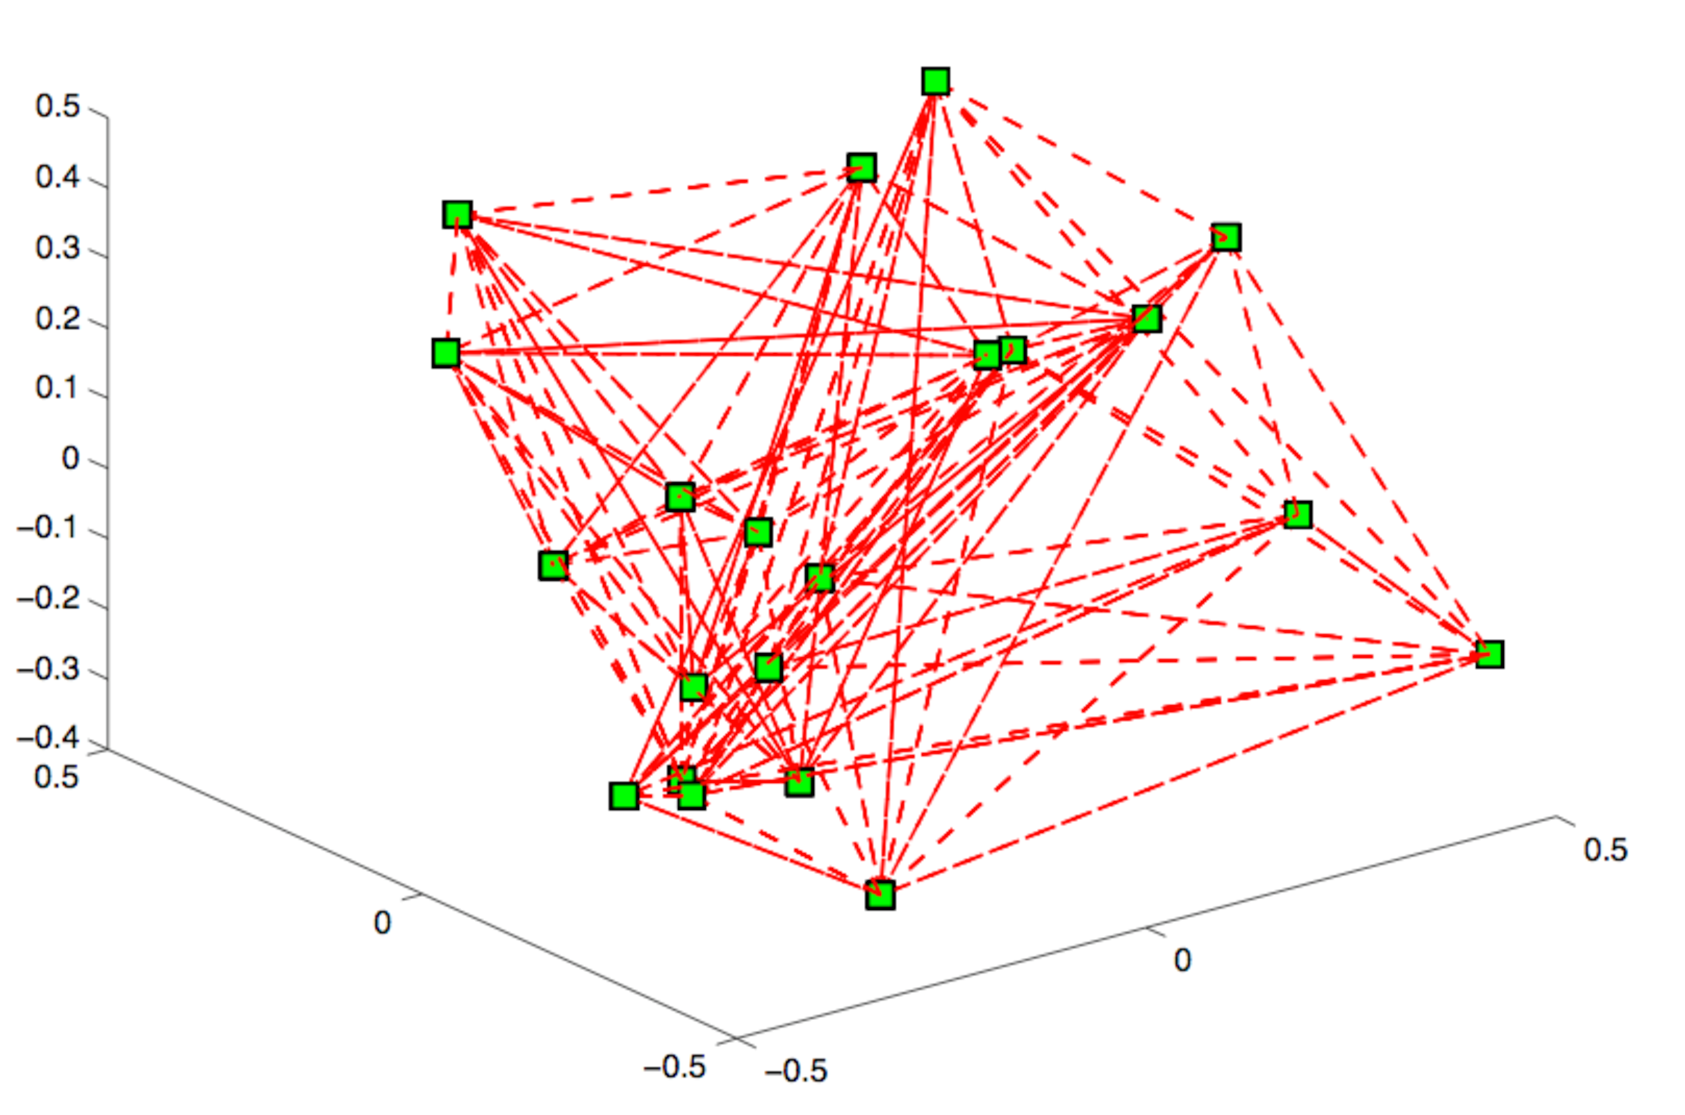
\includegraphics[height=0.34\textheight]{nbody.pdf}
\end{center}

\begin{itemize}
  \item Sources $\y_j$ carry weighted densities.
  \item Targets $\x_i$ may be boundary nodes or field points.
  \item Direct evaluation is $\cO(N^2)$ for $N$ targets and sources.
\end{itemize}
\end{frame}

%================================================================
\begin{frame}{Two viewpoints for fast algorithms}
\small
\begin{columns}[T,totalwidth=\textwidth]
\begin{column}{0.48\textwidth}
\textbf{Algebra-based}
\begin{itemize}\itemsep2pt
  \item Use an exact algebraic identity or matrix factorization.
  \item Examples: FFT and structured matrix factorizations.
  \item When the identity is applied exactly, its numerical error is roundoff.
\end{itemize}
\end{column}
\begin{column}{0.48\textwidth}
\textbf{Analysis-based}
\begin{itemize}\itemsep2pt
  \item Use analytic or geometric structure to construct an approximation.
  \item Examples: FMM, DMK, butterfly, and directional FMM.
  \item The tolerance enters through a controlled numerical rank or expansion.
\end{itemize}
\end{column}
\end{columns}
\vspace{2mm}
\begin{block}{Common question}
How can a dense interaction be represented using a number of degrees of freedom
that is small compared with the number of source--target pairs?
\end{block}
\end{frame}

%================================================================
\begin{frame}{Thread I: low-rank compression}
\small
For source points in $B_S$ and target points in $B_T$, let
\[
  A(B_T,B_S)=\{K(\x_i,\y_j)\}_{\x_i\in B_T,\,\y_j\in B_S}.
\]
The central mechanism is a tolerance-dependent approximation
\[
  A(B_T,B_S)\approx U V^T,\qquad \rank_\eps A(B_T,B_S)=p\ll\min(m,n).
\]
Consequently, a block matvec costs approximately $p(m+n)$ rather than $mn$.

\begin{itemize}
  \item The source of the low rank is method-dependent.
  \item The block geometry, scale, and frequency determine whether $p$ stays
  small.
\end{itemize}
\begin{block}{The rest of this section}
Four examples of the same compression principle, followed by the proxy/check
and recursive mechanisms needed to make it fast.
\end{block}
\end{frame}

%================================================================
\begin{frame}{FMM: low rank from well-separated boxes}
\footnotesize
For a nonoscillatory analytic kernel, a well-separated source--target block
has a small numerical rank:
\[
  A_{TS}=\bigl[K(\x_i,\y_j)\bigr]_{\x_i\in B_T,\,\y_j\in B_S}
  \approx U_T\,S\,V_S^*,
  \qquad \rank_\eps(A_{TS})=p\ll\min(m,n).
\]
The corresponding block matvec is
\[
  A_{TS}q_S\approx U_T\!\left(S\bigl(V_S^*q_S\bigr)\right),
  \qquad \text{cost }\cO\bigl(p(m+n)\bigr)\text{ instead of }\cO(mn).
\]
\begin{center}
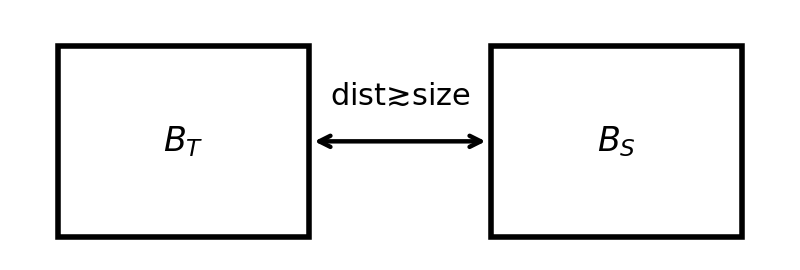
\includegraphics[width=0.75\textwidth]{well_separation_far.png}
\end{center}
\end{frame}

%================================================================
\begin{frame}{DMK: low rank from kernel splitting}
\footnotesize
For the 3D Laplace kernel, the DMK construction uses a hierarchy of scales:
\[
  \frac1r\approx W_0(r)+\sum_{\ell=0}^{L-1}D_\ell(r)+R_L(r),
\]
\[
  W_0(r)\approx\frac{\erf(r/\sigma_0)}{r},\qquad
  D_\ell(r)=\frac{\erf(r/\sigma_{\ell+1})-\erf(r/\sigma_\ell)}{r},
  \qquad
  R_L(r)=\frac{\erfc(r/\sigma_L)}{r},
\]
with $\sigma_0>\sigma_1>\cdots>\sigma_L$.
\begin{itemize}
  \item $D_\ell$ is smooth and negligible beyond colleague boxes at level
  $\ell$ to the requested precision.
  \item A localized Fourier convolution represents its interaction on that
  level with a precision-dependent number of modes; $R_L$ is the local
  residual correction.
  \item The compression comes from the kernel split, not from separation of the
  original kernel block.
\end{itemize}
{\scriptsize\color{mygray}S. Jiang and L. Greengard, ``A dual-space multilevel kernel-splitting framework for discrete and continuous convolution,''
\emph{Commun. Pure Appl. Math.} 78 (2025), 1086--1143.}
\end{frame}

%================================================================
\begin{frame}{Butterfly: complementary low rank}
\small
For an oscillatory kernel such as $K(x,\xi)=e^{2\pi\ii x\xi}$, organize the
row and column indices in two trees, $T_X$ and $T_\Omega$.  At level $\ell$ in
$T_X$ and the complementary level $L-\ell$ in $T_\Omega$,
\[
  K_{A,B}\approx U_A\,M_{A,B}\,V_B^*,
  \qquad \rank_\eps(K_{A,B})\le p(\eps),
\]
where $A$ is a node of $T_X$ at level $\ell$ and $B$ is a node of
$T_\Omega$ at level $L-\ell$.

\begin{itemize}
  \item The source- and target-box widths have a constant product at these
  complementary levels; this is the condition that keeps the rank bounded.
  \item The two trees must therefore be traversed simultaneously; this gives
  the sparse product of factors in a butterfly factorization.
\end{itemize}
{\scriptsize\color{mygray}E. Candes, L. Demanet, and L. Ying, ``Fast computation of Fourier integral operators,''
\emph{SIAM J. Sci. Comput.} 29 (2007); Y. Li, H. Yang, E. R. Martin, K. L. Ho, and L. Ying,
``Butterfly factorization,'' \emph{SIAM Multiscale Model. Simul.} 13 (2015).}
\end{frame}

%================================================================
\begin{frame}{Directional FMM: low rank in a wedge}
\small
For the high-frequency Helmholtz kernel, ordinary separation is not enough.
The directional FMM uses a parabolic separation condition: a source box of
width $w$ interacts with targets in a narrow wedge whose angular width is of
order $1/w$ and whose distance is of order $w^2$ in the nondimensionalized
setting.

For that wedge, the field generated by sources $\{\y_i,f_i\}$ admits a
rank-$p(\eps)$ equivalent-source representation:
\[
  \sum_i G(\x,\y_i)f_i\approx
  \sum_{q=1}^{p}G(\x,\bm{b}_q)\,\widetilde f_q,
  \qquad \x\text{ in the wedge}.
\]

\begin{itemize}
  \item The wedge condition is what keeps $p(\eps)$ bounded at high frequency.
  \item The hierarchy tracks both box scale and propagation direction; this is
  different from the nonoscillatory FMM.
\end{itemize}
{\scriptsize\color{mygray}B. Engquist and L. Ying, ``Fast directional multilevel algorithms for oscillatory kernels,''
\emph{SIAM J. Sci. Comput.} 29 (2007); A. Benson, J. Poulson, K. Tran, B. Engquist, and L. Ying,
``A parallel directional fast multipole method,'' \emph{SIAM J. Sci. Comput.} 36 (2014).}
\end{frame}

%================================================================
\begin{frame}{Thread II: proxy sources and check potentials}
\small
Let $Y$ be a source cluster, $X_{\rm chk}$ a small set of check targets, and
$Y_{\rm prx}$ a small set of proxy sources.  Match the potential of $Y$ at
$X_{\rm chk}$ by choosing proxy strengths $\widetilde q$:
\[
  K(X_{\rm chk},Y)q
  \approx K(X_{\rm chk},Y_{\rm prx})\widetilde q,
\]
For the prescribed far region, the proxy sources then approximate the field:
\[
  K(X_{\rm far},Y)q
  \approx K(X_{\rm far},Y_{\rm prx})\widetilde q.
\]
\begin{itemize}
  \item The proxy and check sets are chosen for the cluster geometry and the
  far region being represented.
  \item Analytic expansions can replace this numerical proxy construction;
  proxy/check representations are the corresponding data-sparse mechanism.
\end{itemize}
\end{frame}

%================================================================
\begin{frame}{Why the proxy set must stay small}
\small
The purpose of proxy or check points is to make the compression stage cheap:
\[
  \text{many sources/targets}
  \longrightarrow
  p\ \text{check values and }p\ \text{proxy degrees of freedom},
  \qquad p\ll N.
\]
\begin{itemize}
  \item If $p$ grows with the number of source or target points in a cluster,
  forming and applying the compressed representation can lose the
  fast-algorithm advantage.
  \item Analytic low-rank expansions avoid sampling the full interaction and
  can be preferable when the kernel structure is known explicitly.
  \item The same idea appears as equivalent sources/check potentials in
  kernel-independent and directional FMM constructions.
\end{itemize}
{\scriptsize\color{mygray}L. Ying, G. Biros, and D. Zorin, ``A kernel-independent adaptive fast multipole method in two and three dimensions,''
\emph{J. Comput. Phys.} 196 (2004); A. Benson et al., \emph{SIAM J. Sci. Comput.} 36 (2014).}
\end{frame}

%================================================================
\begin{frame}{Thread III: recursion makes compression useful}
\small
Low-rank compression applied at only one level leaves most of the dense work
untouched.  Fast algorithms apply it recursively on a hierarchy:
\begin{center}
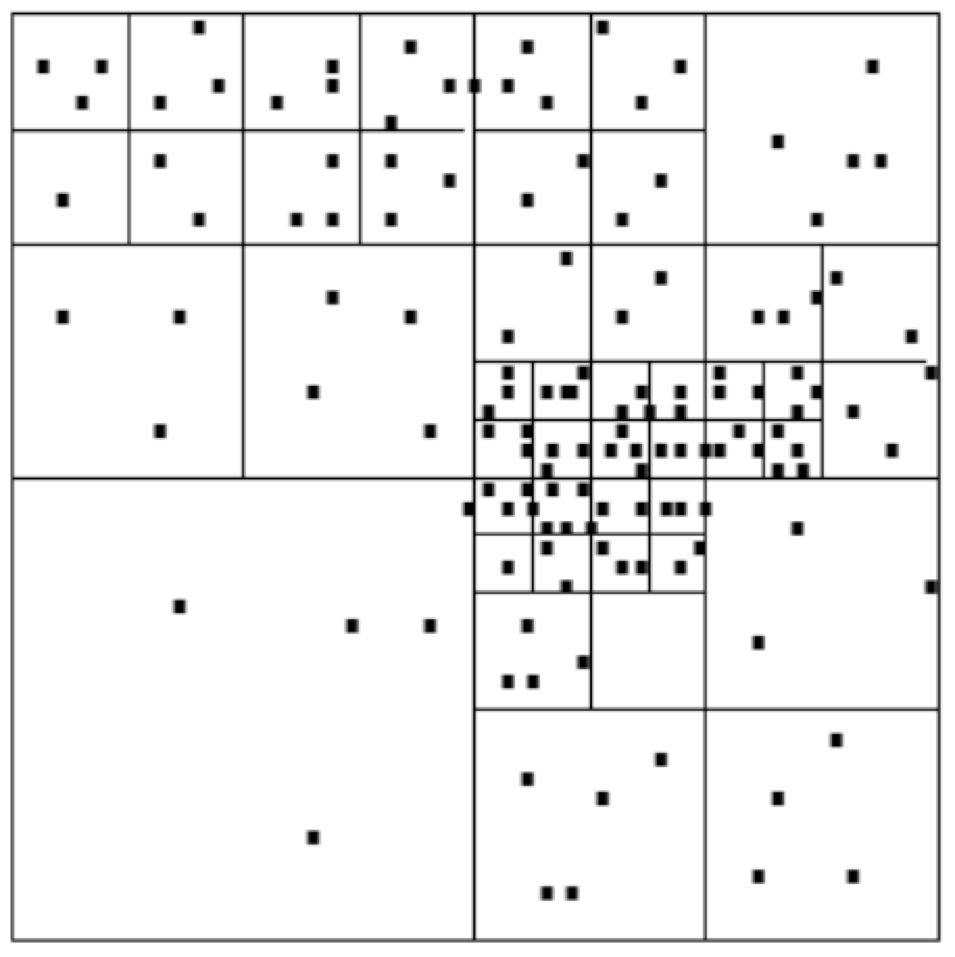
\includegraphics[height=0.31\textheight]{adaptivetree.png}
\end{center}
\begin{itemize}
  \item coarse levels represent long-range or large-scale interactions;
  fine levels resolve smaller scales and local corrections;
  \item the representation is transferred between levels rather than rebuilt
  from all source--target pairs at every level;
  \item under the method-specific rank, geometry, and admissibility assumptions,
  this leads to linear or quasilinear complexity.
\end{itemize}
\end{frame}

%================================================================
\begin{frame}{One recursive pattern, several organizations}
\small
\begin{center}
\renewcommand{\arraystretch}{1.25}
\begin{tabular}{p{0.19\textwidth}p{0.34\textwidth}p{0.32\textwidth}}
\toprule
Method & What is compressed & What is traversed recursively \\
\midrule
FMM & well-separated blocks & spatial box tree \\
DMK & scale-local difference kernels & spatial levels and Fourier representation \\
Butterfly & complementary low-rank blocks & paired source and target trees \\
Directional FMM & directional wedge interactions & spatial tree and directions \\
\bottomrule
\end{tabular}
\end{center}
\vspace{2mm}
\begin{block}{The common architecture}
Low rank supplies the compression; compact coefficient representations make it
efficient; recursion applies it across the hierarchy.
\end{block}
\end{frame}

%================================================================
\begin{frame}{Fast matvec inside a BIE solver}
\small
For one iterative-solver step,
\[
  \bm y=A_N\bm x
  =\alpha\bm x+A_{\rm near}\bm x+A_{\rm compressed}\bm x.
\]
\begin{itemize}
  \item $\alpha\bm x$: local identity or jump term, when present.
  \item $A_{\rm near}$: self and near-panel interactions, including special
  quadrature corrections.
  \item $A_{\rm compressed}$: the far or multiscale part, evaluated by the
  appropriate analysis-based or algebra-based fast method.
\end{itemize}
\begin{block}{Important separation}
The fast method accelerates the dense kernel sum.  It does not replace the
geometry, singular quadrature, close evaluation, or iterative-solver analysis.
\end{block}
\end{frame}

%================================================================
\begin{frame}{Complete fast BIE solver architecture}
\small
A complete fast BIE code must also handle:
\begin{itemize}
  \item geometry refinement and panel bookkeeping;
  \item self and near-panel quadrature;
  \item close target evaluation;
  \item vector/tensor kernels and multiple densities;
  \item iterative solver stopping criteria;
  \item preconditioning or direct solvers when the iteration count is large.
\end{itemize}
\begin{block}{Course perspective}
The compression mechanism is only one component of a reliable integral-equation
solver; the discretization and error budget determine what must be accelerated.
\end{block}
\end{frame}

%================================================================
\begin{frame}{Periodic sums, Ewald, and NUFFT}
\small
Periodic Green's functions and lattice sums introduce a different structure:
\[
\sum_{\bm n\in\mathbb{Z}^d}
K(\x-\y+\bm n L).
\]
Ewald methods split the kernel into
\[
K=K_{\rm real}+K_{\rm Fourier},
\]
with rapid convergence in both parts.

\begin{block}{NUFFT role}
The Fourier part often reduces to evaluating nonuniform trigonometric sums;
this is where NUFFT technology enters.
\end{block}
\end{frame}

%================================================================
\begin{frame}{Fast direct solvers: motivation}
\small
Fast matvec plus GMRES is a natural choice when:
\begin{itemize}
  \item the BIE is well-conditioned;
  \item the number of right-hand sides is small;
  \item no near-nullspace physics slows convergence.
\end{itemize}

Fast direct solvers become attractive when:
\begin{itemize}
  \item there are many right-hand sides;
  \item frequencies or material contrasts make iterations expensive;
  \item a reusable preconditioner/factorization is worth building.
\end{itemize}
\end{frame}

%================================================================
\begin{frame}{Fast direct solvers as preconditioners}
\small
An approximate hierarchical factorization can be used as
\[
M^{-1}A\bm x=M^{-1}\bm b.
\]
Even if $M^{-1}$ is not accurate enough as a direct inverse, it may reduce the
GMRES iteration count substantially.

\begin{block}{Practical use}
This is often an effective compromise for difficult geometries, high contrast,
or frequency regimes where pure second-kind conditioning is insufficient.
\end{block}
\end{frame}

%================================================================
\begin{frame}{Hierarchical matrix compression}
\small
Off-diagonal blocks of elliptic BIE matrices are often low rank:
\[
  A_{ij}\approx U_{ij}V_{ij}^T
  \quad\text{for well-separated index clusters}.
\]
Hierarchical direct solvers exploit this recursively.

\begin{itemize}
  \item HODLR/HSS/HBS matrices.
  \item Recursive skeletonization.
  \item Hierarchical interpolative factorization.
  \item Strong preconditioners from approximate inverses.
\end{itemize}
\end{frame}

%================================================================
\begin{frame}{Interpolative decomposition}
\small
Given a numerically low-rank matrix block $B$,
\[
  B\approx B(:,J)T,
\]
where $J$ selects representative columns.

\begin{block}{Skeletonization interpretation}
Only a subset of degrees of freedom is needed to represent the far-field
interaction of a cluster. These selected degrees of freedom are called
skeletons.
\end{block}
\end{frame}

%================================================================
\begin{frame}{Many right-hand sides}
\small
Suppose one solve costs
\[
T_{\rm iter}=m\,T_{\rm mv}
\]
with GMRES+FMM, and a fast direct method costs
\[
T_{\rm build}+r\,T_{\rm apply}
\]
for $r$ right-hand sides.

\begin{block}{Break-even criterion}
A direct or factorized method becomes attractive when
\[
T_{\rm build}+r\,T_{\rm apply}
<
r\,m\,T_{\rm mv}.
\]
\end{block}

This comparison is relevant when the same discretized operator is reused for
multiple right-hand sides.
\end{frame}

%================================================================
\section{HPC Basics}

\begin{frame}{HPC constraints for fast integral codes}
\small
Fast algorithms are only asymptotic statements until they meet hardware.
\[
  \text{runtime}
  \ne
  \text{flop count only}.
\]

\begin{itemize}
  \item Memory movement can dominate arithmetic.
  \item Tree traversal creates irregular access patterns.
  \item Vectorization requires regular batches.
  \item Threading requires attention to locality and load balance.
  \item GPU acceleration changes the cost model.
\end{itemize}
\end{frame}

%================================================================
\begin{frame}{Asymptotic complexity versus time to solution}
\small
Two algorithms may both be $\cO(N)$ but differ by a large constant:
\[
T(N)=c_{\rm alg}(\eps)\,N+T_{\rm setup}.
\]
On real hardware, $c_{\rm alg}$ depends on
\begin{itemize}
  \item memory bandwidth and cache reuse;
  \item vectorization and instruction mix;
  \item branch divergence and indirect addressing;
  \item communication and synchronization;
  \item batching granularity.
\end{itemize}

\begin{block}{Engineering standard}
Report both scaling and absolute time to solution at a stated accuracy.
\end{block}
\end{frame}

%================================================================
\begin{frame}{Co-design for fast integral codes}
\small
\begin{center}
\begin{tikzpicture}[
  >=Latex,
  every node/.style={font=\scriptsize},
  designnode/.style={draw,thick,align=center,text width=3.0cm,
    minimum height=1.05cm,inner sep=3pt},
  center/.style={draw,thick,align=center,text width=2.6cm,
    minimum height=0.90cm,inner sep=3pt,fill=black!5}
]
  \node[designnode] (method) at (0,2.15)
    {Numerical method\\accuracy\\stability\\complexity};
  \node[designnode] (software) at (-3.2,-0.65)
    {Software\\data layout\\batching\\parallel runtime};
  \node[designnode] (hardware) at (3.2,-0.65)
    {Hardware\\cache\\SIMD/GPU\\memory/network};
  \node[center] (goal) at (0,0.45)
    {time to solution\\at target accuracy};

  \draw[->,thick,SFdark] (method) -- (goal);
  \draw[->,thick,SFdark] (software) -- (goal);
  \draw[->,thick,SFdark] (hardware) -- (goal);
  \draw[<->,thick,black!55] (software) -- node[below] {implementation choices} (hardware);
  \draw[<->,thick,black!55] (method) -- node[left] {discretization} (software);
  \draw[<->,thick,black!55] (method) -- node[right] {cost model} (hardware);
\end{tikzpicture}
\end{center}
\vspace{-0.8em}
\begin{block}{Design principle}
A fast algorithm becomes an efficient solver only when the discretization,
data structures, and target hardware are designed together.
\end{block}
\end{frame}

%================================================================
\begin{frame}{What does FLOP/s measure?}
\small
\begin{itemize}
  \item A \emph{floating-point operation} is one arithmetic operation such as
        addition or multiplication.
  \item For a timed computation,
    \[
      \text{achieved FLOP/s}
      = \frac{\text{number of counted FLOPs}}{\text{elapsed time}}.
    \]
  \item FLOP/s is a hardware-performance metric; it does not by itself
        measure accuracy or time to solution.
\end{itemize}
\begin{block}{For matrix multiplication}
For $C\leftarrow AB$, with $A\in\mathbb{R}^{M\times K}$ and
$B\in\mathbb{R}^{K\times N}$, count $2MNK$ FLOPs.
\end{block}
\end{frame}

%================================================================
\begin{frame}{Theoretical peak FLOP rate}
\small
\footnotesize
\begin{itemize}\setlength{\itemsep}{0pt}
  \item \textbf{FMA} means \emph{fused multiply-add}: $a\leftarrow bc+a$.
        It counts as two floating-point operations, one multiplication and one
        addition.
  \item \textbf{SIMD} means \emph{single instruction, multiple data}: one
        instruction applies the same arithmetic operation to several values.
  \item A 512-bit vector register holds $512/64=8$ double-precision values,
        because one double-precision value occupies 64 bits.
\end{itemize}

For the Intel Skylake server-core model used in the source benchmark, the
peak-rate estimate is
\[
  \begin{aligned}
  &(2\ \text{FMA units})
  \times(8\ \text{double values per SIMD instruction})\\[-1mm]
  &\quad\times(2\ \text{FLOPs per FMA})
  \times(3.3\ \text{GHz})
  =105.6\ \text{GFLOP/s}.
  \end{aligned}
\]
\small
\begin{itemize}\setlength{\itemsep}{0pt}
  \item This is an upper bound under the stated hardware assumptions.
  \item A benchmark reports how much of that bound a particular kernel reaches.
\end{itemize}
\begin{block}{Important distinction}
Peak FLOP/s is computed from hardware capabilities; achieved FLOP/s is
computed from a timed implementation.
\end{block}
\vspace{-0.45em}
\tiny Source: D. Malhotra (2022); hardware model and assumptions shown above.
\end{frame}

%================================================================
\begin{frame}{Measuring achieved FLOP/s with GEMM}
\footnotesize
\textbf{GEMM} means general matrix--matrix multiplication.  It computes
\[
  C\leftarrow AB,
  \qquad A\in\mathbb{R}^{M\times K},\quad
  B\in\mathbb{R}^{K\times N},\quad
  C\in\mathbb{R}^{M\times N}.
\]
\textbf{BLAS} (Basic Linear Algebra Subprograms) provides standard kernels
such as matrix multiplication; \textbf{LAPACK} builds higher-level dense
linear-algebra algorithms from BLAS.

Repeat a fixed-size kernel many times so timer overhead is negligible:
\[
  \text{FLOP rate}=\frac{2MNK\,L}{T},
\]
where $L$ is the number of repetitions and $T$ is the measured time.
\begin{itemize}\setlength{\itemsep}{0pt}
  \item Start with the direct triple loop.
  \item Then expose SIMD parallelism and unroll independent work.
  \item In the example below, $M=N=K=8$; we compare the achieved rate with
        the same peak estimate.
\end{itemize}
\begin{block}{Lesson for fast integral codes}
The operation count is not enough: data layout, instruction dependencies,
vectorization, and reuse determine the measured rate.
\end{block}
\end{frame}

%================================================================
\begin{frame}[fragile]{GEMM micro-kernel: direct implementation}
\small
\begin{columns}[T]
\column{0.49\textwidth}
\begin{block}{Column-major direct kernel}
\tiny\ttfamily
\begin{verbatim}
for (int k = 0; k < K; ++k)
  for (int j = 0; j < N; ++j)
    for (int i = 0; i < M; ++i)
      C[i+j*M] += A[i+k*M] * B[k+K*j];
\end{verbatim}
\end{block}
\vspace{-0.4em}
Each innermost update performs one multiplication and one addition.  A timed
run of $L$ repetitions reports $2MNKL/T$ FLOP/s.

\column{0.48\textwidth}
\begin{center}
\begin{tikzpicture}[scale=0.72]
  \fill[CCMorange!28] (0,0) rectangle (1.5,-1.5);
  \draw[step=0.25,black!45] (0,0) grid (1.5,-1.5);
  \node at (0.75,-0.75) {$C$};
  \node at (1.9,-0.75) {$=$};
  \fill[SFdark!18] (2.4,0) rectangle (4.25,-1.5);
  \draw[step=0.25,black!45] (2.4,0) grid (4.25,-1.5);
  \node at (3.325,-0.75) {$A$};
  \node at (4.65,-0.75) {$\times$};
  \fill[green!20] (5.15,0) rectangle (6.65,-1.85);
  \draw[step=0.25,black!45] (5.15,0) grid (6.65,-1.85);
  \node at (5.9,-0.925) {$B$};
  \node[align=center] at (3.35,-2.35)
    {$C\in\R^{M\times N},\ A\in\R^{M\times K},\ B\in\R^{K\times N}$};
\end{tikzpicture}
\end{center}
\end{columns}
\end{frame}

%================================================================
\begin{frame}[fragile]{GEMM micro-kernel: vectorized implementation}
\small
\begin{columns}[T]
\column{0.60\textwidth}
\begin{block}{Vectorized kernel}
\tiny\ttfamily
\begin{verbatim}
Vec C_vec[N];
for (int j = 0; j < N; ++j)
  C_vec[j] = Vec::Load(C+j*M);

for (int k = 0; k < K; ++k) {
  const Vec A_vec = Vec::Load(A+k*M);
  for (int j = 0; j < N; ++j)
    C_vec[j] = A_vec * B[k+K*j] + C_vec[j];
}

for (int j = 0; j < N; ++j)
  C_vec[j].Store(C+j*M);
\end{verbatim}
\end{block}

\column{0.34\textwidth}
\footnotesize
\begin{itemize}\setlength{\itemsep}{0.35em}
  \item `Vec` represents one SIMD vector of double-precision values.
  \item The code loads a vector of entries of $A$ and updates a vector of
        entries of $C$ at once.
  \item The mathematics is unchanged; only the instruction grouping changes.
\end{itemize}
\end{columns}
\end{frame}

%================================================================
\begin{frame}[fragile]{GEMM micro-kernel: unrolling and throughput}
\small
\begin{columns}[T]
\column{0.48\textwidth}
\begin{block}{Loop-unrolled kernel}
\tiny\ttfamily
\begin{verbatim}
#pragma GCC unroll (8)
for (int k = 0; k < K; ++k) {
  const Vec A_vec = Vec::Load(A+k*M);
  #pragma GCC unroll (8)
  for (int j = 0; j < N; ++j)
    C_vec[j] = A_vec * B[k+K*j] + C_vec[j];
}
\end{verbatim}
\end{block}
\vspace{-0.2em}
Unrolling presents several independent vector FMA operations to the processor.

\column{0.48\textwidth}
For $M=N=K=8$:
\begin{center}
\resizebox{\columnwidth}{!}{%
\begin{tabular}{lcc}
\toprule
implementation & GFLOP/s & peak fraction\\
\midrule
naive & 5.99578 & 5.7\%\\
vectorized & 29.3319 & 27.8\%\\
vectorized + unrolled & 38.5658 & 36.5\%\\
\bottomrule
\end{tabular}
}
\end{center}
\begin{block}{Point of the example}
The operation count is unchanged, while the measured throughput changes by
more than a factor of six.
\end{block}
\scriptsize
Source: D. Malhotra, \textit{What Every Programmer Should Know About High
Performance Computing} (2022).
\end{columns}
\end{frame}

%================================================================
\begin{frame}{Instruction-level parallelism}
\small
Modern processors execute independent operations concurrently through
pipelines and vector units.
\begin{itemize}
  \item A long dependency chain limits throughput even when the arithmetic is
        simple.
  \item Reorganizing equivalent arithmetic can expose independent operations.
  \item SIMD treats several scalar values as one vector operation; regular
        loops and structure-of-arrays layouts help the compiler use it.
\end{itemize}
\begin{block}{Example}
Polynomial evaluation makes the dependency structure visible: Horner's rule
is compact, while Estrin's method exposes more independent subexpressions.
\end{block}
\end{frame}

%================================================================
\begin{frame}{Polynomial evaluation: Horner's rule}
\small
For
\[
  p(x)=a_0+a_1x+\cdots+a_7x^7,
\]
Horner's rule evaluates
\[
  p(x)=(((((((a_7x+a_6)x+a_5)x+a_4)x+a_3)x+a_2)x+a_1)x+a_0).
\]
\begin{itemize}
  \item The arithmetic is compact: one multiply-add per coefficient after
        initialization.
  \item Each step depends on the previous step, so the recurrence has a long
        dependency chain.
\end{itemize}
\end{frame}

%================================================================
\begin{frame}{How to read the polynomial pipeline schedules}
\footnotesize
We use the following timing model for a pipelined vector multiply-add
instruction:
\begin{itemize}\setlength{\itemsep}{0pt}
  \item \textbf{Clock cycle:} one tick of the processor clock.
  \item \textbf{Vector FMA latency:} A vector FMA has four-cycle latency. In
        the one-based schedule used below, an instruction issued in cycle $j$
        occupies cycles $j$ through $j+3$; a dependent FMA can issue in cycle
        $j+4$.
  \item \textbf{Throughput:} the two vector FMA units can begin two
        independent vector multiply-adds per clock cycle.
\end{itemize}
\begin{center}
\begin{tikzpicture}[x=0.68cm,y=0.48cm,
  every node/.style={font=\scriptsize}]
  \foreach \j in {1,...,7}
    \node at (\j-0.5,4.0) {\j};
  \node[anchor=east] at (0,4.0) {cycle};
  \foreach \s/\y in {1/3,2/2,3/1,4/0}
    \node[anchor=east] at (0,\y+0.35) {stage \s};
  \foreach \x/\label/\fill in {0/A/CCMorange!35,1/B/SFdark!18,2/C/green!25,3/D/CCMorange!55,4/E/SFdark!35,5/F/green!38,6/G/CCMorange!75}
    \draw[fill=\fill] (\x,3) rectangle ++(1,0.7) node[midway] {\label};
  \foreach \x/\label/\fill in {1/A/CCMorange!35,2/B/SFdark!18,3/C/green!25,4/D/CCMorange!55,5/E/SFdark!35,6/F/green!38}
    \draw[fill=\fill] (\x,2) rectangle ++(1,0.7) node[midway] {\label};
  \foreach \x/\label/\fill in {2/A/CCMorange!35,3/B/SFdark!18,4/C/green!25,5/D/CCMorange!55,6/E/SFdark!35}
    \draw[fill=\fill] (\x,1) rectangle ++(1,0.7) node[midway] {\label};
  \foreach \x/\label/\fill in {3/A/CCMorange!35,4/B/SFdark!18,5/C/green!25,6/D/CCMorange!55}
    \draw[fill=\fill] (\x,0) rectangle ++(1,0.7) node[midway] {\label};
\end{tikzpicture}
\end{center}
\begin{center}
$A,B,C,\ldots$ are independent FMAs issued on one pipeline.  These schedules
measure dependent-arithmetic latency, not memory-access latency.
\end{center}
\end{frame}

%================================================================
\begin{frame}{Horner's rule: dependency chain and pipeline}
\small
\begin{columns}[T]
\column{0.58\textwidth}
\begin{center}
\resizebox{0.84\textwidth}{!}{%
\begin{tikzpicture}[nodes={draw,circle,inner sep=1.5pt,font=\scriptsize},
  edge from parent/.style={draw,{Latex[length=1.4mm]}-}]
\node {$\times,+$}
  child { node {$\times,+$}
    child { node {$\times,+$}
      child { node {$\times,+$}
        child { node {$\times,+$}
          child { node {$\times,+$}
            child { node {$\times,+$}
              child { node {$a_7$} }
              child { node {$x$} }
              child { node {$a_6$} }
            }
            child { node {$x$} }
            child { node {$a_5$} }
          }
          child { node {$x$} }
          child { node {$a_4$} }
        }
        child { node {$x$} }
        child { node {$a_3$} }
      }
      child { node {$x$} }
      child { node {$a_2$} }
    }
    child { node {$x$} }
    child { node {$a_1$} }
  }
  child { node {$x$} }
  child { node {$a_0$} };
\end{tikzpicture}}
\end{center}

\column{0.38\textwidth}
\scriptsize
\begin{center}
\resizebox{\linewidth}{!}{%
\begin{tabular}{c c c}
\toprule
operation & FMA unit & issue $\to$ ready\\
\midrule
$u=a_7x+a_6$ & FMA1 & $1\to4$\\
$v=ux+a_5$ & FMA1 & $5\to8$\\
$w=vx+a_4$ & FMA1 & $9\to12$\\
$\cdots$ & FMA1 & $\cdots$\\
$p(x)$ & FMA1 & $25\to28$\\
\bottomrule
\end{tabular}
}
\end{center}
Each result is needed by the next operation, so the next FMA issues four
cycles later:
\[
  7\ \text{stages}\times4\ \text{cycles/stage}=28\ \text{cycles}.
\]
FMA2 is idle. Thus the issue utilization of the two FMA units is
\[
  \frac{7}{28\times2}=12.5\%.
\]
\end{columns}
\end{frame}

%================================================================
\begin{frame}{Polynomial evaluation: Estrin's method}
\small
Group neighboring terms to expose independent subexpressions:
\[
\begin{aligned}
p(x)={}&((a_7x+a_6)x^2+(a_5x+a_4))x^4\\
       &+(a_3x+a_2)x^2+(a_1x+a_0).
\end{aligned}
\]
Compute $x^2$, $x^4$, and the four linear combinations in parallel, then
combine them.
\begin{itemize}
  \item Estrin uses more temporary values and multiplications.
  \item The shorter dependency depth can improve throughput on a superscalar
        or vector processor.
\end{itemize}
\end{frame}

%================================================================
\begin{frame}[t]{Estrin evaluation: two FMA pipelines}
\small
\begin{columns}[T]
\column{0.43\textwidth}
\footnotesize
\textbf{Operation definitions}\par
\vspace{0.15em}
The colored arrow identifies the instruction entering a pipeline stage.
\[
\begin{aligned}
\textcolor{estrinXtwo}{x^2=x\,x}&\only<1-4>{\leftarrow}\\
\textcolor{estrinXfour}{x^4=x^2x^2}&\only<5-8>{\leftarrow}\\
\textcolor{estrinU}{u=a_7x+a_6}&\only<1-4>{\leftarrow}\\
\textcolor{estrinV}{v=a_5x+a_4}&\only<2-5>{\leftarrow}\\
\textcolor{estrinW}{w=a_3x+a_2}&\only<2-5>{\leftarrow}\\
\textcolor{estrinP}{p=a_1x+a_0}&\only<3-6>{\leftarrow}\\
\textcolor{estrinQ}{q=ux^2+v}&\only<6-9>{\leftarrow}\\
\textcolor{estrinR}{r=wx^2+p}&\only<7-10>{\leftarrow}\\
\textcolor{estrinFinal}{p(x)=qx^4+r}&\only<11-14>{\leftarrow}
\end{aligned}
\]

\column{0.53\textwidth}
\footnotesize
\textbf{Four-stage FMA pipelines}\par
\vspace{0.15em}
Each click advances a colored instruction by one stage; it exits after stage 4.
\begin{center}
\begin{tikzpicture}[x=1.08cm,y=0.75cm,
  every node/.style={font=\footnotesize}]
  \node[anchor=east] at (-0.1,1.35) {FMA2};
  \node[anchor=east] at (-0.1,0.35) {FMA1};
  \foreach \j in {0,...,3} {
    \draw[fill=black!3] (\j,1) rectangle ++(1,0.65);
    \draw[fill=black!3] (\j,0) rectangle ++(1,0.65);
    \node at (\j+0.5,-0.25) {\the\numexpr\j+1\relax};
  }
  \node[anchor=north] at (2,-0.46) {pipeline stage};
  \only<1>{\draw[fill=estrinXtwo] (0,0) rectangle ++(1,0.65);}
  \only<2>{\draw[fill=estrinXtwo] (1,0) rectangle ++(1,0.65);}
  \only<3>{\draw[fill=estrinXtwo] (2,0) rectangle ++(1,0.65);}
  \only<4>{\draw[fill=estrinXtwo] (3,0) rectangle ++(1,0.65);}
  \only<5>{\draw[fill=estrinXfour] (0,0) rectangle ++(1,0.65);}
  \only<6>{\draw[fill=estrinXfour] (1,0) rectangle ++(1,0.65);}
  \only<7>{\draw[fill=estrinXfour] (2,0) rectangle ++(1,0.65);}
  \only<8>{\draw[fill=estrinXfour] (3,0) rectangle ++(1,0.65);}
  \only<1>{\draw[fill=estrinU] (0,1) rectangle ++(1,0.65);}
  \only<2>{\draw[fill=estrinU] (1,1) rectangle ++(1,0.65);}
  \only<3>{\draw[fill=estrinU] (2,1) rectangle ++(1,0.65);}
  \only<4>{\draw[fill=estrinU] (3,1) rectangle ++(1,0.65);}
  \only<2>{\draw[fill=estrinV] (0,0) rectangle ++(1,0.65);}
  \only<3>{\draw[fill=estrinV] (1,0) rectangle ++(1,0.65);}
  \only<4>{\draw[fill=estrinV] (2,0) rectangle ++(1,0.65);}
  \only<5>{\draw[fill=estrinV] (3,0) rectangle ++(1,0.65);}
  \only<2>{\draw[fill=estrinW] (0,1) rectangle ++(1,0.65);}
  \only<3>{\draw[fill=estrinW] (1,1) rectangle ++(1,0.65);}
  \only<4>{\draw[fill=estrinW] (2,1) rectangle ++(1,0.65);}
  \only<5>{\draw[fill=estrinW] (3,1) rectangle ++(1,0.65);}
  \only<3>{\draw[fill=estrinP] (0,0) rectangle ++(1,0.65);}
  \only<4>{\draw[fill=estrinP] (1,0) rectangle ++(1,0.65);}
  \only<5>{\draw[fill=estrinP] (2,0) rectangle ++(1,0.65);}
  \only<6>{\draw[fill=estrinP] (3,0) rectangle ++(1,0.65);}
  \only<6>{\draw[fill=estrinQ] (0,0) rectangle ++(1,0.65);}
  \only<7>{\draw[fill=estrinQ] (1,0) rectangle ++(1,0.65);}
  \only<8>{\draw[fill=estrinQ] (2,0) rectangle ++(1,0.65);}
  \only<9>{\draw[fill=estrinQ] (3,0) rectangle ++(1,0.65);}
  \only<7>{\draw[fill=estrinR] (0,0) rectangle ++(1,0.65);}
  \only<8>{\draw[fill=estrinR] (1,0) rectangle ++(1,0.65);}
  \only<9>{\draw[fill=estrinR] (2,0) rectangle ++(1,0.65);}
  \only<10>{\draw[fill=estrinR] (3,0) rectangle ++(1,0.65);}
  \only<11>{\draw[fill=estrinFinal] (0,0) rectangle ++(1,0.65);}
  \only<12>{\draw[fill=estrinFinal] (1,0) rectangle ++(1,0.65);}
  \only<13>{\draw[fill=estrinFinal] (2,0) rectangle ++(1,0.65);}
  \only<14>{\draw[fill=estrinFinal] (3,0) rectangle ++(1,0.65);}
\end{tikzpicture}
\end{center}
\only<15>{%
\textbf{Completion:} the final FMA starts in cycle 11 and exits the fourth
stage after cycle 14.}
\end{columns}
\end{frame}

%================================================================
\begin{frame}{Making Estrin's independent work explicit}
\small
Both forms below evaluate the same degree-seven polynomial,
\[
  p(x)=a x^7+b x^6+c x^5+d x^4+e x^3+f x^2+g x+h.
\]
\begin{columns}[T,onlytextwidth]
\column{0.48\textwidth}
\begin{block}{Direct Estrin form}
\[
\begin{aligned}
x_2&=x^2, \qquad x_4=x_2^2,\\
p(x)&=\big((ax+b)x_2+(cx+d)\big)x_4\\
&\quad +(ex+f)x_2+(gx+h).
\end{aligned}
\]
The grouping exposes the polynomial as a function of $x^2$ and $x^4$.
\end{block}
\column{0.48\textwidth}
\begin{block}{Expanded Estrin form}
\[
\begin{aligned}
u&=ax+b, &v&=cx+d,\\
w&=ex+f, &z&=gx+h,\\
q&=ux_2+v, &r&=wx_2+z,\\
p(x)&=qx_4+r.
\end{aligned}
\]
The expanded form gives names to independent intermediate results.  It does
not change the polynomial or the Estrin grouping.
\end{block}
\end{columns}
The preceding pipeline diagram is the schedule for these named quantities:
$u,w$ may begin together, as may the independent work used to form $v,z$.
\end{frame}

%================================================================
\begin{frame}{Critical-path latency is an ideal model}
\small
\begin{block}{Critical-path latency model}
The diagrams assume two FMA pipelines and a four-cycle delay before an FMA
result can be used by a dependent instruction.  They count only the longest
chain of arithmetic dependencies:
\[
  \text{Horner: }28\text{ cycles},
  \qquad
  \text{Estrin: }14\text{ cycles}.
\]
This predicts a factor-two reduction in ideal dependency latency.
\end{block}
\begin{block}{Interpretation}
The $28/14$ comparison estimates the delay imposed by the arithmetic
dependencies.  It is not yet a prediction of the elapsed time of a compiled
program: source code, compiler output, and processor execution are not part
of this simplified model.

\smallskip
Horner has one long dependent chain.  Estrin creates independent intermediate
quantities, so two FMA pipelines can work concurrently before their results
must be combined.
\end{block}
\end{frame}

%================================================================
\begin{frame}{From arithmetic to memory movement}
\small
\begin{itemize}
  \item A kernel can be limited by arithmetic throughput or by moving data
        through the memory hierarchy.
  \item Reuse data in registers and caches before returning to main memory.
  \item Blocking and batching make reuse explicit; regular access patterns
        also make SIMD execution easier.
\end{itemize}
\begin{block}{Connection to fast integral algorithms}
Tree interactions, translation operators, and quadrature corrections should be
organized into regular batches whenever the numerical method permits it.
\end{block}
\end{frame}

%================================================================
\begin{frame}{HPC checklist for a fast kernel}
\small
\begin{enumerate}
  \item Count the operations and state the convention.
  \item Measure elapsed time over enough repetitions.
  \item Compare achieved FLOP/s with the relevant peak estimate.
  \item Inspect dependency chains, SIMD use, data layout, and memory reuse.
  \item Report accuracy and time to solution separately from hardware metrics.
\end{enumerate}
\begin{block}{Course message}
Fast asymptotic complexity is necessary, but the implementation must also
expose parallel arithmetic and reuse data effectively.
\end{block}
\end{frame}

%================================================================
\begin{frame}{Practical software stack}
\small
\[
\begin{aligned}
&\text{geometry/chunking}
\rightarrow
\text{quadrature}
\rightarrow
\text{kernel evaluation}\\
&\rightarrow
\text{fast algorithm}
\rightarrow
\text{linear solver}
\rightarrow
\text{field evaluation}.
\end{aligned}
\]

\begin{block}{Course software map}
Chunkie handles geometry/discretization; FMM2D/FMM3D/FMM3DBIE accelerate
kernel sums; FINUFFT and DMK handle Fourier/kernel-splitting primitives;
FLAM illustrates fast direct solver methods.
\end{block}
\end{frame}

%================================================================
\section{Synthesis}

\begin{frame}{One complete model workflow}
\small
\begin{enumerate}
  \item State the BVP and its boundary data.
  \item Choose a Green's function satisfying the PDE and far-field condition.
  \item Choose a layer potential representation.
  \item Take the appropriate boundary limits, including jump terms when
  present, to obtain a BIE.
  \item Verify uniqueness and conditioning.
  \item Discretize geometry and density.
  \item Use singular and near-singular quadrature.
  \item Solve the dense system with GMRES+FMM/DMK or a fast direct solver.
  \item Evaluate the field with close-evaluation corrections.
\end{enumerate}
\end{frame}

%================================================================
\begin{frame}{Key points}
\small
\begin{itemize}
  \item Green's functions solve the PDE analytically away from sources.
  \item Layer potentials move unknowns to the boundary.
  \item Jump relations turn boundary conditions into integral equations.
  \item Singular quadrature is part of the method, not an implementation detail.
  \item FMM, DMK, and fast direct solvers can reduce the cost of dense BIE
  computations when their structural assumptions apply.
  \item HPC constraints determine whether the asymptotic speedup is realized.
\end{itemize}
\end{frame}

%================================================================
\begin{frame}{Selected references}
\footnotesize
\begin{itemize}
  \item R. Kress, \emph{Linear Integral Equations}, 3rd ed., Springer, 2014.
  \item D. Colton and R. Kress, \emph{Integral Equation Methods in Scattering Theory}, Wiley, 1983.
  \item L. Greengard and V. Rokhlin, ``A fast algorithm for particle simulations,'' \emph{Journal of Computational Physics} 73 (1987), 325--348.
  \item S. Jiang and L. Greengard, ``A dual-space multilevel kernel-splitting framework for discrete and continuous convolution,'' \emph{Communications on Pure and Applied Mathematics} 78 (2025), 1086--1143.
  \item P.-G. Martinsson, \emph{Fast Direct Solvers for Elliptic PDEs}, SIAM, 2019.
  \item D. Malhotra, \emph{What Every Programmer Should Know About High Performance Computing}, course slides, 2022.
\end{itemize}
\end{frame}

%================================================================
\begin{frame}{Connections to later topics}
\small
\begin{itemize}
  \item Day 1 afternoon: chunkie and first Nystr\"om solvers.
  \item Day 2: singular quadrature and RCIP.
  \item Day 3: NUFFT, Ewald, DMK, and FMM.
  \item Day 4: volume potentials, function extension, Poisson solvers, RRQ.
  \item Day 5: fast direct solvers and inverse scattering.
  \item Advanced applications: heat/Navier--Stokes and SKIE mode calculation.
\end{itemize}

\begin{block}{Connection to later topics}
The purpose is to give every later method a place in the BVP-to-solver pipeline.
\end{block}
\end{frame}

\end{document}
